\documentclass[11pt]{article}
\usepackage[utf8]{inputenc}
\usepackage[T1]{fontenc}
\usepackage[margin=1.0in]{geometry}
\usepackage{amsmath,amssymb}
\usepackage{graphicx}
\usepackage{booktabs}
\usepackage{array}
\usepackage{xcolor}
\usepackage{listings}
\usepackage{caption}
\usepackage[round,authoryear]{natbib}
\usepackage{hyperref}

\definecolor{codebg}{HTML}{F6F8FA}
\definecolor{codeframe}{HTML}{D0D7DE}
\definecolor{codekw}{HTML}{0550AE}
\definecolor{codecmt}{HTML}{57606A}
\definecolor{linkblue}{HTML}{1F4E78}

\hypersetup{
    colorlinks=true,
    linkcolor=linkblue,
    citecolor=linkblue,
    urlcolor=linkblue
}

\captionsetup{font=small,labelfont=bf,skip=4pt}
\emergencystretch=1.5em

\lstset{
    basicstyle=\ttfamily\footnotesize,
    backgroundcolor=\color{codebg},
    frame=single,
    rulecolor=\color{codeframe},
    breaklines=true,
    keywordstyle=\color{codekw}\bfseries,
    commentstyle=\color{codecmt}\itshape,
    showstringspaces=false,
    tabsize=2,
    aboveskip=6pt,
    belowskip=6pt
}

% Dynamically generated statistical macros from Python pipeline
% Auto-generated by paper2_brainimation/generate_figures.py — DO NOT EDIT MANUALLY
\newcommand{\MuseBrowserKB}{37.4}
\newcommand{\LegacyMuseKB}{473.0}
\newcommand{\BundleReductionFactor}{12.6}
\newcommand{\NRefSensors}{53}
\newcommand{\NRefPFive}{38}
\newcommand{\NRefInput}{27}
\newcommand{\NRefEEGData}{19}
\newcommand{\NRefSound}{16}
\newcommand{\StudioPPGLOCMedian}{211}
\newcommand{\StudioIMULOCMedian}{215}
\newcommand{\StudioMultiLOCMedian}{120}
\newcommand{\NGamesAndEEGEdu}{43}
\newcommand{\BrainGamesLOCMedian}{514}
\newcommand{\NArchivalTotal}{121}
\newcommand{\NeurotechLOCMedian}{149}
\newcommand{\NeuroArtLOCMedian}{43}
\newcommand{\NAdditionalSketches}{26}
\newcommand{\NStarterDiag}{7}
\newcommand{\StarterDiagLOCMedian}{25}
\newcommand{\StarterDiagLOCIQRLow}{22}
\newcommand{\StarterDiagLOCIQRHigh}{120}
\newcommand{\StarterDiagLOCMin}{21}
\newcommand{\StarterDiagLOCMax}{135}
\newcommand{\NStudiosGroup}{27}
\newcommand{\StudiosLOCMedian}{208}
\newcommand{\StudiosLOCIQRLow}{136}
\newcommand{\StudiosLOCIQRHigh}{257}
\newcommand{\StudiosLOCMin}{69}
\newcommand{\StudiosLOCMax}{1438}
\newcommand{\GamesEEGEduLOCMedian}{131}
\newcommand{\GamesEEGEduLOCIQRLow}{38}
\newcommand{\GamesEEGEduLOCIQRHigh}{438}
\newcommand{\GamesEEGEduLOCMin}{17}
\newcommand{\GamesEEGEduLOCMax}{758}
\newcommand{\ArchivalLOCMedian}{126}
\newcommand{\ArchivalLOCIQRLow}{50}
\newcommand{\ArchivalLOCIQRHigh}{174}
\newcommand{\ArchivalLOCMin}{12}
\newcommand{\ArchivalLOCMax}{414}
\newcommand{\StuClusterLOCMin}{87}
\newcommand{\StuClusterLOCMax}{302}
\newcommand{\WilcoxonEpochsW}{435.0}
\newcommand{\WilcoxonEpochsP}{1.86 \times 10^{-9}}
\newcommand{\EpochsExpansionFactor}{2.07}
\newcommand{\NCatalogueSketches}{234}
\newcommand{\NCatalogueCategories}{21}
\newcommand{\CatLOCMedian}{110}
\newcommand{\CatLOCIQRLow}{38}
\newcommand{\CatLOCIQRHigh}{183}
\newcommand{\CatLOCMin}{11}
\newcommand{\CatLOCMax}{1438}
\newcommand{\NPPGSketches}{11}
\newcommand{\NIMUSketches}{11}
\newcommand{\NMultiSketches}{5}
\newcommand{\NBrainGames}{14}
\newcommand{\NEEGEduModules}{13}
\newcommand{\NClassicEEGEdu}{16}
\newcommand{\NNeurotechCatalogue}{95}
\newcommand{\NNeuroArtGallery}{26}
\newcommand{\ERPNoiseRMSKOne}{17.4}
\newcommand{\ERPNoiseRMSKFive}{5.7}
\newcommand{\ERPNoiseRMSKTwenty}{2.7}
\newcommand{\ERPMCNoiseRMSKOne}{13.8}
\newcommand{\ERPMCNoiseRMSKFive}{6.1}
\newcommand{\ERPMCNoiseRMSKTwenty}{3.1}
\newcommand{\ERPSMEKOne}{8.7}
\newcommand{\ERPSMEKFive}{3.6}
\newcommand{\ERPSMEKTwenty}{1.9}
\newcommand{\ERPBlinkPtPUV}{166.2}
\newcommand{\ERPBlinkPThreeHundredBiasUV}{6.7}
\newcommand{\ERPRMSECleanTwentyUV}{3.04}
\newcommand{\ERPRMSEBlinkUnrejectedUV}{4.52}
\newcommand{\ERPRMSEBlinkRejectedUV}{3.33}
\newcommand{\JitterFCMSixteenHz}{26.6}
\newcommand{\JitterFCThirtyHz}{14.8}
\newcommand{\JitterFCFortyFiveHz}{9.8}
\newcommand{\JitterNullThirtyHz}{33.3}
\newcommand{\JitterNullFortyFiveHz}{22.2}
\newcommand{\JitterRetNarrowPct}{65.5}
\newcommand{\JitterRetNOneSeventyPct}{94.7}
\newcommand{\JitterRetPThreeHundredPct}{98.9}
\newcommand{\JitterPThreePeakLatSDMS}{31.5}
\newcommand{\JitterPThreeAreaLatSDMS}{10.4}
\newcommand{\JitterPThreeTempLatSDMS}{13.4}
\newcommand{\AperiodicExpRelaxed}{1.41}
\newcommand{\AperiodicExpActive}{1.07}
\newcommand{\AlphaPeakAboveOneFRelDB}{8.5}
\newcommand{\AlphaPeakAboveOneFActDB}{2.4}
\newcommand{\AlphaRawDiffDB}{5.4}
\newcommand{\AlphaAdjDiffDB}{6.2}
\newcommand{\ERPSNRKOne}{0.55}
\newcommand{\ERPSNRKFive}{1.66}
\newcommand{\ERPSNRKTwenty}{3.48}
\newcommand{\EMAVarReductionPct}{98.4}
\newcommand{\FNIRSErrRawUM}{1.15}
\newcommand{\FNIRSErrCleanUM}{0.11}
\newcommand{\FNIRSErrRawUMThreeD}{1.147}
\newcommand{\FNIRSErrCleanUMThreeD}{0.113}
\newcommand{\FNIRSSuppDB}{20.1}
\newcommand{\FNIRSRRaw}{0.46}
\newcommand{\FNIRSRClean}{0.99}
\newcommand{\NLMSRMSERawUV}{43.7}
\newcommand{\NLMSRMSECleanUV}{4.8}
\newcommand{\NLMSSuppDB}{19.2}
\newcommand{\NLMSRRaw}{0.31}
\newcommand{\NLMSRClean}{0.95}
\newcommand{\HEPTrueWinMeanUV}{1.64}
\newcommand{\HEPTruePeakUV}{4.27}
\newcommand{\HEPSMEUV}{0.79}
\newcommand{\HEPSurrCIUV}{3.12}
\newcommand{\HEPPermP}{0.0200}
\newcommand{\NLMSLagThirtyOneOneTapDB}{2.4}
\newcommand{\NLMSLagThirtyOneFourTapDB}{11.0}
\newcommand{\NLMSLagThirtyOneGainDB}{8.6}
\newcommand{\NBuiltinExamples}{36}
\newcommand{\NBuiltinCategories}{10}
\newcommand{\NRefAPIs}{153}
\newcommand{\NRefGroups}{30}
\newcommand{\NRefTabs}{5}
\newcommand{\ExLOCMedian}{32}
\newcommand{\ExLOCIQRLow}{27}
\newcommand{\ExLOCIQRHigh}{36}
\newcommand{\ExLOCMin}{11}
\newcommand{\ExLOCMax}{111}
\newcommand{\NStudentSketches}{69}
\newcommand{\NUniqueStudents}{30}
\newcommand{\StuClusterLOCMedian}{164}
\newcommand{\StuClusterLOCIQRLow}{122}
\newcommand{\StuClusterLOCIQRHigh}{173}
\newcommand{\MannWhitneyU}{2437.0}
\newcommand{\MannWhitneyClusterU}{1074.0}
\newcommand{\RankBiserialClusterR}{0.99}
\newcommand{\StuLOCMedian}{155}
\newcommand{\StuLOCMean}{157.5}
\newcommand{\StuLOCSD}{65.7}
\newcommand{\StuLOCIQRLow}{116}
\newcommand{\StuLOCIQRHigh}{189}
\newcommand{\StuLOCMin}{38}
\newcommand{\StuLOCMax}{378}
\newcommand{\NStuNF}{40}
\newcommand{\StuNFLOCMedian}{121}
\newcommand{\StuNFLOCIQRLow}{99}
\newcommand{\StuNFLOCIQRHigh}{171}
\newcommand{\StuNFLOCMin}{38}
\newcommand{\StuNFLOCMax}{378}
\newcommand{\NStuERP}{29}
\newcommand{\StuERPLOCMedian}{176}
\newcommand{\StuERPLOCIQRLow}{153}
\newcommand{\StuERPLOCIQRHigh}{221}
\newcommand{\StuERPLOCMin}{117}
\newcommand{\StuERPLOCMax}{306}
\newcommand{\StuPctCond}{66.7}
\newcommand{\StuCntCond}{46}
\newcommand{\StuPctAlpha}{53.6}
\newcommand{\StuCntAlpha}{37}
\newcommand{\StuPctRaw}{39.1}
\newcommand{\StuCntRaw}{27}
\newcommand{\StuPctBeta}{42.0}
\newcommand{\StuCntBeta}{29}
\newcommand{\StuPctERP}{42.0}
\newcommand{\StuCntERP}{29}
\newcommand{\StuPctAtt}{34.8}
\newcommand{\StuCntAtt}{24}
\newcommand{\StuPctTheta}{29.0}
\newcommand{\StuCntTheta}{20}
\newcommand{\StuPctParticles}{49.3}
\newcommand{\StuCntParticles}{34}
\newcommand{\StuPctMed}{26.1}
\newcommand{\StuCntMed}{18}
\newcommand{\StuPctAudio}{13.0}
\newcommand{\StuCntAudio}{9}
\newcommand{\StuPctEvents}{15.9}
\newcommand{\StuCntEvents}{11}
\newcommand{\NFPctCond}{57.5}
\newcommand{\NFCntCond}{23}
\newcommand{\ERPPctCond}{79.3}
\newcommand{\ERPCntCond}{23}
\newcommand{\NFPctAlpha}{92.5}
\newcommand{\NFCntAlpha}{37}
\newcommand{\ERPPctAlpha}{0.0}
\newcommand{\ERPCntAlpha}{0}
\newcommand{\NFPctBeta}{72.5}
\newcommand{\NFCntBeta}{29}
\newcommand{\ERPPctBeta}{0.0}
\newcommand{\ERPCntBeta}{0}
\newcommand{\NFPctRaw}{0.0}
\newcommand{\NFCntRaw}{0}
\newcommand{\ERPPctRaw}{93.1}
\newcommand{\ERPCntRaw}{27}
\newcommand{\NFPctAtt}{52.5}
\newcommand{\NFCntAtt}{21}
\newcommand{\ERPPctAtt}{10.3}
\newcommand{\ERPCntAtt}{3}
\newcommand{\NFPctParticles}{70.0}
\newcommand{\NFCntParticles}{28}
\newcommand{\ERPPctParticles}{20.7}
\newcommand{\ERPCntParticles}{6}
\newcommand{\CatCntAlpha}{132}
\newcommand{\CatPctAlpha}{56.4}
\newcommand{\CatCntBeta}{96}
\newcommand{\CatPctBeta}{41.0}
\newcommand{\CatCntAtt}{76}
\newcommand{\CatPctAtt}{32.5}
\newcommand{\CatCntTheta}{75}
\newcommand{\CatPctTheta}{32.1}
\newcommand{\CatCntRaw}{44}
\newcommand{\CatPctRaw}{18.8}
\newcommand{\CatCntIMU}{39}
\newcommand{\CatPctIMU}{16.7}
\newcommand{\CatCntAudio}{18}
\newcommand{\CatPctAudio}{7.7}
\newcommand{\CatCntPPG}{19}
\newcommand{\CatPctPPG}{8.1}

\raggedbottom

\title{\textbf{BrainImation: Bringing Brain Waves to Life in the Browser with Affordable Muse Headbands}}

\author{
\parbox{0.94\textwidth}{\centering
\textbf{Kyle E. Mathewson}$^{\text{a,b,*}}$, \textbf{Tamari Shalamberidze}$^{\text{a}}$, \textbf{Claire J. Scavuzzo}$^{\text{a}}$\\[5pt]
\footnotesize $^{\text{a}}$Department of Psychology, Faculty of Science, University of Alberta, Edmonton, AB, T6G 2E9, Canada\\
\footnotesize $^{\text{b}}$Neuroscience and Mental Health Institute, University of Alberta, Edmonton, AB, T6G 2E1, Canada\\
\footnotesize $^*$Correspondence: \texttt{kyle.mathewson@ualberta.ca} \ $\cdot$ \ \texttt{shalambe@ualberta.ca} \ $\cdot$ \ \texttt{scavuzzo@ualberta.ca}\\
\footnotesize Live Tool: \url{https://kylemath.github.io/Brainimation/}\\
Repository: \url{https://github.com/kylemath/Brainimation}
}
}

\date{}

\begin{document}
\maketitle

\begin{abstract}
We present BrainImation (\url{https://kylemath.github.io/Brainimation/}), a free, zero-install browser environment designed for neuroscience and psychology educators, students, and researchers that connects four generations of InteraXon Muse headbands (Muse 2016, Muse~2, Classic Muse~S, and Muse~S Athena) directly to interactive graphics and audio synthesis in a single webpage (\texttt{p5.js}, \texttt{p5.sound}). To eliminate operating-system driver and software-installation barriers in university courses, a built-in WebBluetooth client pairs with a hardware-free signal simulator to populate a single shared signal object providing filtered and raw 4-channel EEG, frequency-band powers, forehead optical pulse and blood oxygenation (PPG/fNIRS), and 3D head motion, supported by a visual catalogue of runnable examples and a click-to-insert API reference drawer (\MuseBrowserKB~KB client, \BundleReductionFactor$\times$ smaller than legacy bundles; \NCatalogueSketches\ sketches across \NCatalogueCategories\ categories, starting from \NStarterDiag\ one-sensor starters/diagnostics and \NBuiltinExamples\ core scaffolds of median \ExLOCMedian\ lines of code [LOC]; \NRefAPIs\ reference items). Deterministic simulation benchmarks illustrate four teaching modules: (1) converting EEG rhythms into sound and separating a periodic alpha peak from the $1/f$ aperiodic background, (2) averaging trials into an event-related potential (ERP), rejecting large artifacts, and estimating peak latency, (3) separating a deeper prefrontal blood-oxygen change from the skin pulse, and (4) removing head-movement artifacts from the EEG. In an upper-level undergraduate cognitive neuroscience laboratory course, students with minimal prior coding experience expanded the short starter templates into complete closed-loop neurofeedback games and 4-channel ERP experiments ($N = \NStudentSketches$ graded examination projects from $N_{\text{students}} = \NUniqueStudents$ learners).\\[4pt]
\noindent\textbf{Keywords:} electroencephalography (EEG); functional near-infrared spectroscopy (fNIRS); photoplethysmography (PPG); brain--computer interface (BCI); event-related potential (ERP); neuroscience and psychology education
\end{abstract}

\clearpage
\setcounter{tocdepth}{3}
\tableofcontents
\clearpage

\section{Introduction}

\subsection{Classroom \& Research Motivation}

\subsubsection{Closed-Loop BCIs \& Neurofeedback}
Closed-loop brain--computer interfaces (BCIs) and neurofeedback systems translate ongoing brain, cardiac, and movement signals into real-time visual or auditory feedback, allowing participants to observe internal physiological states or control interactive displays \citep{sitaram2017closed,enriquez2017eeg,lotte2013flaws}. Closed-loop BCIs can also be used in a university classroom, where neuroscience and psychology lecturers allow students to record and respond to live physiological signals. This turns abstract textbook topics, such as oscillatory brain rhythms, phasic alertness and cognitive control \citep{dekleijn2023short,dekleijn2025phasic}, sensory and cognitive evoked potentials, neurovascular coupling, and movement artifacts, into concrete, hands-on experiments \citep{mathewson2024moving,miranda2014brain,janssen2021opportunities}.

\subsubsection{Headbands vs.\ Pre-Built Dashboards}
Over the past two decades, open-source analysis toolboxes \citep{delorme2004eeglab,makowski2021neurokit2,cannard2024brainbeats}, affordable dry-electrode EEG headbands, and portable computing hardware have made it practical to record human brain activity in undergraduate teaching laboratories and naturalistic settings rather than electrically shielded research suites \citep{krigolson2017choosing,mathewson2017high,kuziek2017transitioning,kuziek2018increasing,cannard2021validating,sabio2024scoping,vanbueren2026comparing}. In parallel, browser-based teaching dashboards such as \emph{EEGEdu} (\url{https://eegedu.com}) \citep{mathewson2026eegedu} allow instructors to demonstrate live brain waves, frequency spectra, and event-related averages through ready-made interactive charts. Once students grasp those foundational displays, however, a natural instructional challenge arises: how can neuroscience and psychology educators help students with little or no programming experience move from passively viewing pre-built graphs to designing and coding their own closed-loop neurofeedback tasks, auditory sonifications, prefrontal blood-oxygen visualizers, and event-related potential (ERP) experiments?

\begin{figure}[t!]
\centering
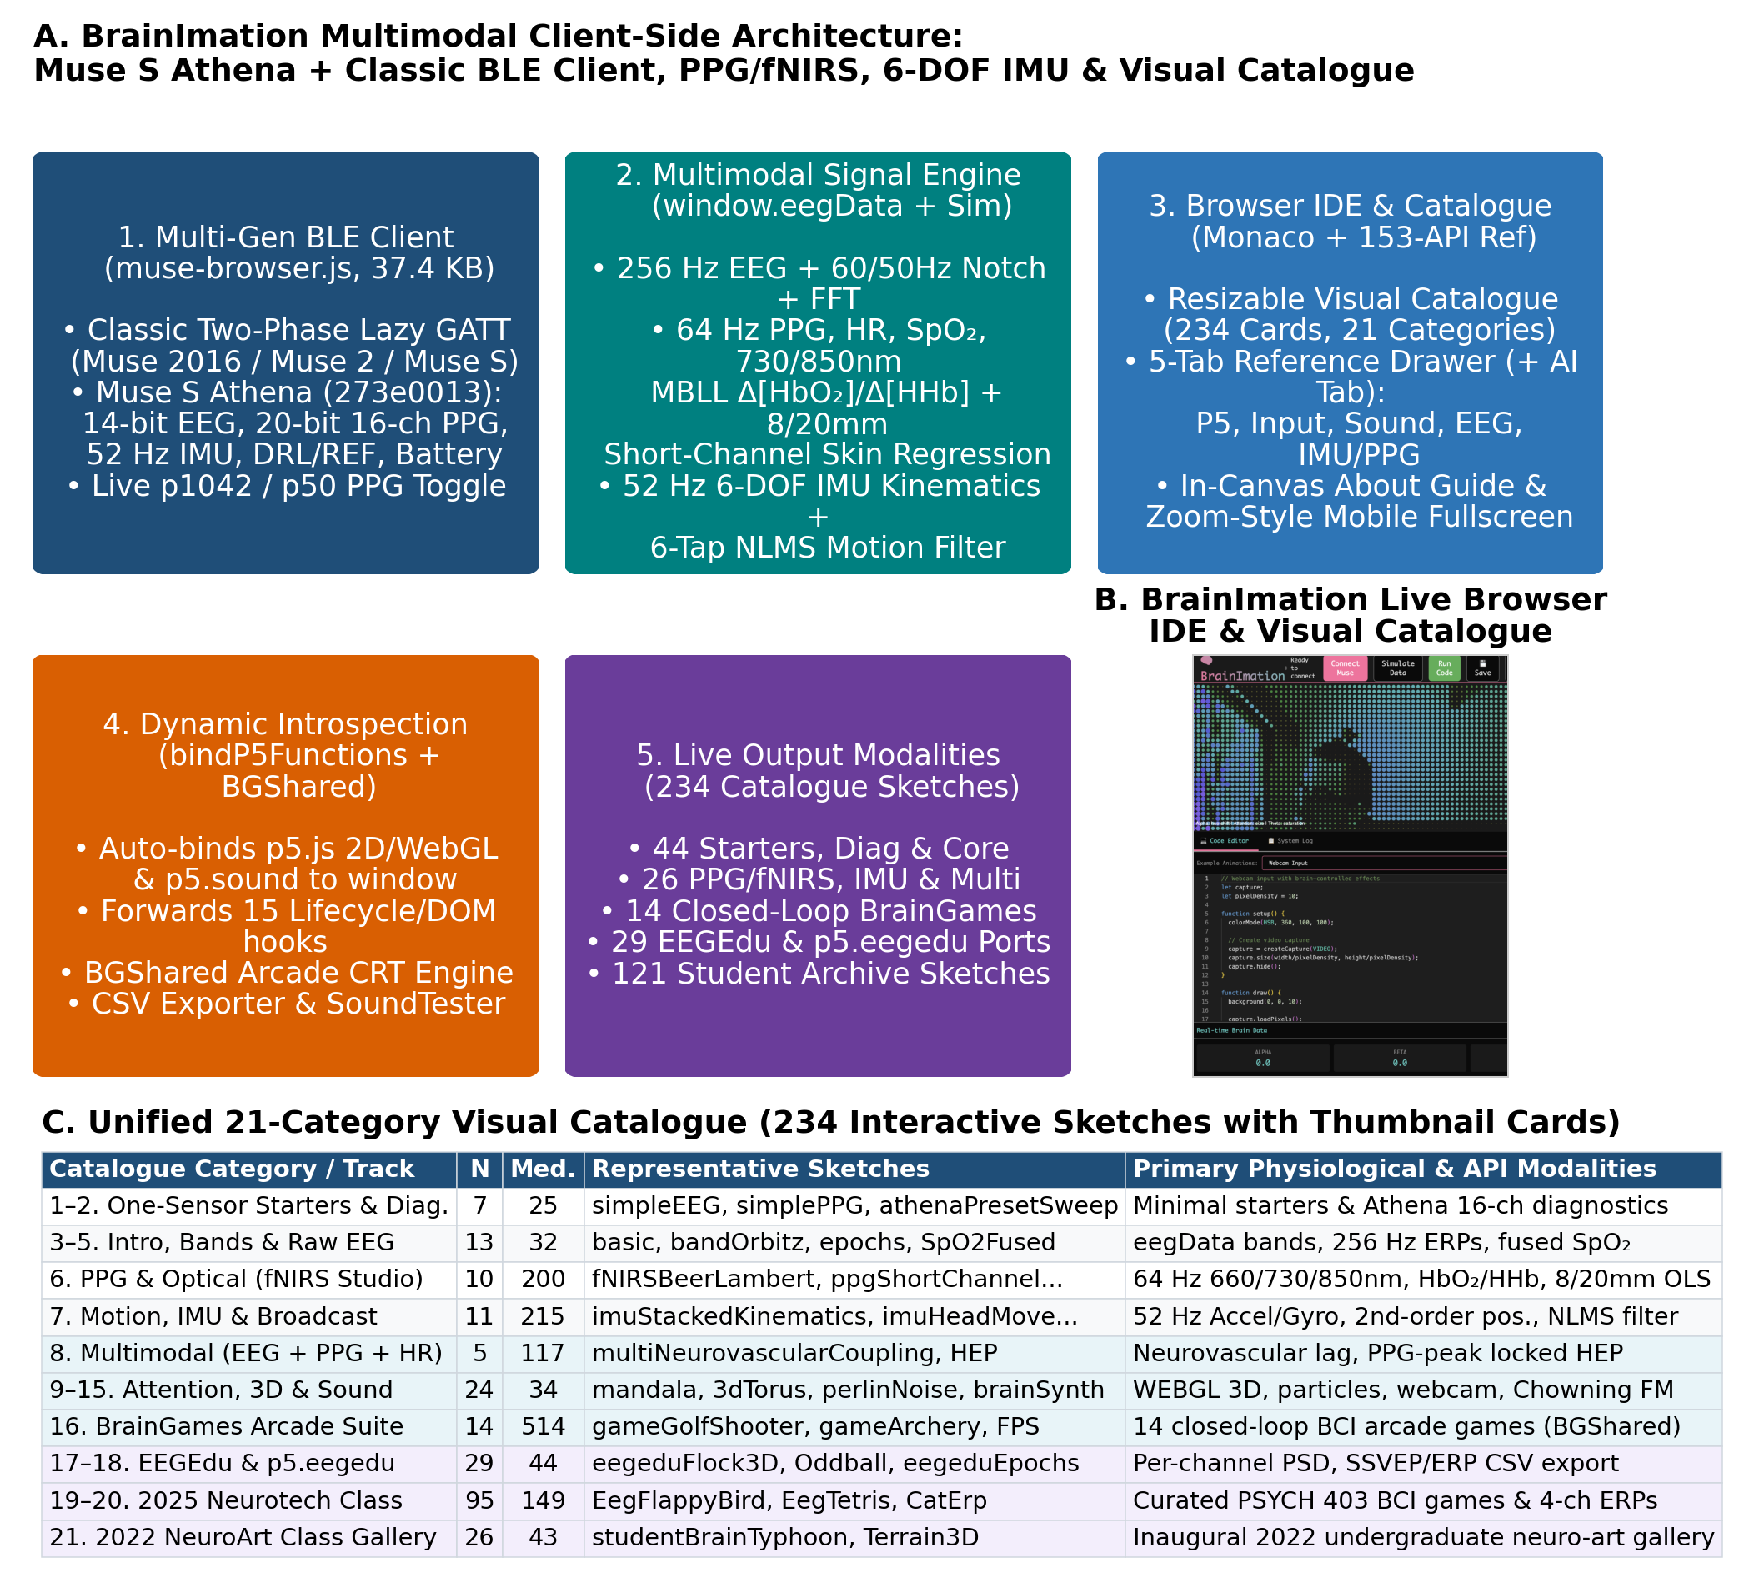
\includegraphics[width=0.98\textwidth]{figures/fig1_equal_boxes.pdf}
\caption{\textbf{BrainImation Classroom Coding Environment and \NCatalogueCategories-Category Visual Catalogue (\NCatalogueSketches\ Sketches).} \textbf{(A)} Overview of the browser workflow: a built-in WebBluetooth client for Muse 2016, Muse~2, Classic Muse~S, and Muse~S Athena headbands pairs with a hardware-free signal simulator to populate a shared signal object (EEG, optical PPG/fNIRS, and 6-axis head motion; \texttt{eegData}), which drives user sketches in the split-screen code editor at 60~FPS. \textbf{(B)} The BrainImation browser interface with the Visual Catalogue open. \textbf{(C)} Summary of the \NCatalogueSketches\ teaching examples and student projects organized across \NCatalogueCategories\ categories.}
\label{fig:ide}
\end{figure}

\subsection{Constructionist Design \& Setup Barriers}

\subsubsection{Constructionist Design Goals}
Widely adopted creative-coding and behavioral-science platforms such as \texttt{Processing} \citep{reas2007processing}, \texttt{Scratch} \citep{resnick2009scratch}, \texttt{p5.js} \citep{mccarthy2015p5}, \texttt{jsPsych} \citep{deleeuw2015jspsych,deleeuw2023simulating,deleeuw2024datapipe}, and \texttt{lab.js} \citep{henninger2022labjs} follow a constructionist learning philosophy \citep{papert1980mindstorms}: students learn computational and scientific methods most effectively when an environment combines a ``low floor'' (allowing beginners to run a meaningful first program within minutes), a ``high ceiling'' (supporting full multi-condition laboratory experiments as skills grow), and ``wide walls'' (accommodating diverse student projects across cognitive neuroscience, experimental psychology, biofeedback games, and media art). In behavioral and perception research, browser-based toolkits have transformed how instructors and investigators build online tasks \citep{woods2015conducting}, measure visual attention via cursor-aperture tracking \citep{dalmaijer2022mouseview}, estimate psychometric thresholds \citep{pronk2023jsquestplus}, stream born-open behavioral datasets \citep{deleeuw2024datapipe}, and simulate synthetic participant behavior so researchers and students can verify experimental logic and analysis pipelines before testing human participants \citep{deleeuw2023simulating}.

\subsubsection{Eliminating Desktop Dependencies}
Extending that same zero-install browser workflow to live physiological recording has historically been difficult. In research laboratories, multimodal synchronization and physiological preprocessing are well served by desktop middleware such as the Lab Streaming Layer \citep{kothe2025lsl}, mobile brain/body imaging pipelines \citep{klug2022bemobil}, Python neurophysiological toolboxes such as \texttt{NeuroKit2} \citep{makowski2021neurokit2}, EEGLAB cardiovascular plugins such as \texttt{BrainBeats} \citep{cannard2024brainbeats}, and synchronous multimodal web viewers \citep{pijalek2026meedav}. In an undergraduate classroom, however, even a simple live exercise, such as scaling the size of a circle on screen with alpha band power ($8\text{--}12\text{ Hz}$), forehead blood oxygenation, or head tilt, typically requires installing an operating-system Bluetooth utility, streaming data over a local network socket, running a background Python or MATLAB script to filter and epoch the data, and forwarding values to a separate display window. Troubleshooting operating-system permissions, package versions, and broken network streams across dozens of student laptops routinely consumes entire laboratory periods before students can engage with the neuroscience itself.

\subsubsection{Classroom Neuroimaging Lessons}
Recent pedagogical work in undergraduate neuroscience education has underscored both the enthusiasm students bring to live physiological recording and the value of structured coding scaffolds \citep{janssen2021opportunities,hatton2023quantitative,smith2024lowcost,iemi2026icancode}. For example, \citet{hatton2023quantitative} showed that pairing qualitative wave inspection with quantitative spectral analysis across consumer and teaching EEG setups deepens students' conceptual understanding of both introductory and advanced neurophysiology, while \citet{smith2024lowcost} designed accessible classroom and laboratory exercises that guide undergraduates through both continuous brain rhythms and event-related potentials on low-cost hardware. Complementing hardware laboratories, \citet{iemi2026icancode} demonstrated through their ``I Can Code'' workshop that introducing neuroscience students to programming within the direct context of brain data substantially boosts coding self-efficacy, and \citet{clindeffarges2026socrates} recently used wearable brain sensing to compare Socratic questioning against direct AI instruction during interactive learning. BrainImation builds directly on these educational advances by uniting live multi-generation headband streaming, hardware-free simulation \citep{deleeuw2023simulating}, and scaffolded creative coding inside a single browser tab.

\subsection{BrainImation Overview \& Minimal Example}

\subsubsection{Browser-Native Hardware \& Simulator}
To provide a zero-install starting point for both neuroscience and psychology instruction and rapid research prototyping, we developed BrainImation (\url{https://github.com/kylemath/Brainimation}), a browser-based coding environment that connects four generations of InteraXon Muse headbands (Muse 2016, Muse~2, Classic Muse~S, and Muse~S Athena) directly to live graphics and Web Audio synthesis inside a single webpage \citep{mccarthy2015p5} (Figure~\ref{fig:ide}; \texttt{p5.js}, \texttt{p5.sound}).

\subsubsection{11-Line Neurofeedback}
By opening a single web link in a Chromium browser, an instructor or student can pair a physical Muse headband \citep{krigolson2017choosing,kuziek2017transitioning,kuziek2018increasing}, or click the built-in signal simulator button in any browser when working at home without hardware, and run a complete closed-loop neurofeedback animation in just \ExLOCMin~lines of JavaScript (\texttt{examples/basic.js}):

\noindent\begin{minipage}{\textwidth}
\begin{lstlisting}
function setup() {
  colorMode(HSB, 360, 100, 100);
}
function draw() {
  background(0, 0, 10);
  let size = map(eegData.alpha, 0, 1, 50, 300);
  let hue = map(eegData.attention, 0, 1, 180, 360);
  fill(hue, 80, 90);
  noStroke();
  ellipse(width/2, height/2, size, size);
}
\end{lstlisting}
\end{minipage}
\vspace{4pt}

The remainder of this paper explains how BrainImation is organized and how it can be used in neuroscience and psychology courses. Section~2 describes how the built-in Bluetooth client connects all four Muse headset generations and how live and simulated streams converge into a single shared signal object. Section~3 presents the classroom coding supports, including the \NRefAPIs-item Reference Drawer and the \NCatalogueSketches-sketch Visual Catalogue across \NCatalogueCategories\ categories. Section~4 walks through four core teaching modules: audio sonification, online ERP trial averaging, optical fNIRS short-channel skin regression, and 3D head-motion integration with adaptive artifact filtering. These modules pair readable JavaScript examples with simulation benchmarks that illustrate why each signal-processing step is needed. Finally, Section~5 evaluates $N = \NStudentSketches$ examination projects authored by $N_{\text{students}} = \NUniqueStudents$ undergraduate students in an upper-level cognitive neuroscience laboratory course, and Section~6 discusses practical guidelines and limitations for classroom and laboratory adoption.

\section{Browser Hardware \& Simulation}

\subsection{Multi-Generation Muse Client}

\subsubsection{Mixed Classroom Headband Fleets}
University neuroscience and psychology teaching laboratories commonly maintain mixed fleets of older and newer headbands purchased across several academic years. All four headbands use the same four dry EEG electrodes: TP9 and TP10 behind the ears, and AF7 and AF8 on the forehead. The reference and ground sit on the center of the forehead. Muse~2 and Classic Muse~S add a forehead optical pulse sensor. Muse~S Athena adds a short (8 mm) and a long (20 mm) optical channel, so a skin pulse can be separated from a deeper blood-oxygen signal. Every model also carries a 6-axis motion sensor.

A major practical obstacle for browser-based instruction is that older WebBluetooth libraries only connect reliably to the original Muse 2016 headband (\texttt{muse-js}): they fail during connection on Muse~2 and Classic Muse~S headsets, which require an explicit wake-up command before turning on their sensor streams, and they cannot decode the newer Muse~S Athena, which packs all of its sensors into a single combined data stream. To let students and instructors pair whichever headband is on the lab bench without installing external software, BrainImation includes a compact, self-contained WebBluetooth client (Table~\ref{tab:gatt}; \MuseBrowserKB~KB, \BundleReductionFactor$\times$ smaller than legacy bundles; \texttt{muse-browser.js}).

\begin{table}[t!]
\centering
\caption{\textbf{Comparison of Desktop LSL Setups, Legacy Browser \texttt{muse-js}, and BrainImation's Built-In Browser Client (\texttt{muse-browser.js}).}}
\label{tab:gatt}
\footnotesize
\setlength{\tabcolsep}{5pt}
\begin{tabular}{p{0.18\textwidth}p{0.23\textwidth}p{0.23\textwidth}p{0.28\textwidth}}
\toprule
\textbf{Feature} & \textbf{Desktop LSL (\texttt{muselsl}+Py)} & \textbf{Legacy \texttt{muse-js} (v3.0)} & \textbf{BrainImation (\texttt{muse-browser.js})} \\
\midrule
Setup Required & OS BLE + Python + LSL & $\LegacyMuseKB\text{ KB}$ (\texttt{RxJS} bundle) & $\MuseBrowserKB\text{ KB}$ (No install, $\BundleReductionFactor\times$ smaller) \\
Connection Flow & Native desktop app & Single-step (fails on Muse 2/S) & Two-Step Wake-Up + Athena Decoder \\
Muse 2016 & Supported & Supported (EEG only) & Supported (EEG, IMU, Battery) \\
Muse 2 / Classic S & OS-dependent & Fails to connect & Supported (EEG, 3-Ch PPG, IMU) \\
Muse S Athena & Unsupported & Unsupported & Supported (EEG, Dual-Distance PPG/fNIRS, IMU, DRL/REF) \\
Built-In Simulator & None (Hardware req.) & Single-channel demo & 4-Ch EEG + Dual-Distance PPG/fNIRS + 3D Head Motion \\
\bottomrule
\end{tabular}
\end{table}

\subsubsection{Two-Step Wake-Up \& Athena}
When a user clicks the Bluetooth button in the top toolbar, the client automatically detects whether the paired headband is a Classic Muse (Muse 2016, Muse~2, or Classic Muse~S) or a Muse~S Athena. For Classic Muse headsets, the client first opens the control channel, sends a preset command and a start command to wake up the onboard sensors, and then subscribes to the separate EEG, forehead optical pulse (PPG), motion (accelerometer and gyroscope), and battery streams. For the Muse~S Athena, the client subscribes to the headset's combined stream and unpacks the tagged sensor packets for 4- or 8-channel EEG, multi-wavelength 16-channel forehead optical readings (verified via hardware diagnostic scripts as Red $660\text{ nm}$, Ambient, Near-Infrared $730\text{ nm}$, and Infrared $850\text{ nm}$ light across short $8\text{ mm}$ and long $20\text{ mm}$ source--detector spacings; \texttt{tools/}), 6-axis head motion, forehead reference voltages, and battery level. The top toolbar also provides a one-click optical toggle button so instructors and students can turn the forehead optical sensors on during blood-flow and fNIRS lessons or switch the LEDs off during EEG-only exercises (\texttt{muse.setPPGMode(enabled)}; presets \texttt{p1042}/\texttt{p50} vs.\ \texttt{p1035}/\texttt{p21}):

\noindent\begin{minipage}{\textwidth}
\begin{lstlisting}
// Simplified two-step connection flow in muse-browser.js
// Step 1: Connect control channel first, then wake up sensor streams
this.controlChar = await this.service.getCharacteristic(CONTROL_CHAR_UUID);
await this.sendCommand('h');      // Halt previous stream
await this.sendCommand(preset);   // 'p50' (Classic EEG+PPG) or 'p1042' (Athena 16-ch optics)
await this.sendCommand('s');      // Start streaming so sensor channels appear
await this.delay(500);

// Step 2: Subscribe to Classic Muse channels or Muse S Athena combined stream (273e0013)
const chars = await this.service.getCharacteristics();
if (chars.some(c => c.uuid.includes('273e0013'))) {
  athenaChar.addEventListener('characteristicvaluechanged', e => this.parseAthenaNotification(e));
} else {
  this.bindClassicMuseStreams(chars); // EEG (256 Hz), PPG (64 Hz), IMU (52 Hz), Telemetry
}
\end{lstlisting}
\end{minipage}
\vspace{4pt}

\subsection{Shared Signal State \& Simulator}

\subsubsection{Unified Signal State Object}
A core pedagogical design principle of BrainImation is that student code should run identically whether driven by a physical headband in the teaching lab or by the built-in signal simulator on a personal laptop at home \citep{deleeuw2023simulating}. Both the Bluetooth client and the simulator write their live values into the same shared signal object, which organizes real-time measurements into five intuitive sensor groups accessible inside the main animation loop (\texttt{EEGSimulator}; \texttt{window.eegData}; \texttt{draw()}).

\subsubsection{Frequency Bands \& ERP Buffers}
For frequency-band neurofeedback, the shared signal object provides continuous power estimates scaled between $0.0$ and $1.0$ across the five standard EEG frequency bands: delta ($1\text{--}4\text{ Hz}$), theta ($4\text{--}8\text{ Hz}$), alpha ($8\text{--}12\text{ Hz}$), beta ($13\text{--}30\text{ Hz}$), and gamma ($30\text{--}50\text{ Hz}$). Each band is available both as a whole-head average and individually across the two behind-the-ear temporal electrodes and two forehead electrodes (\texttt{TP9}, \texttt{AF7}, \texttt{AF8}, \texttt{TP10}; \citealp{cannard2021validating,sabio2024scoping}). During live headband recordings, the incoming 256~Hz EEG signal first passes through an automatic filter chain that removes electrical wall-outlet hum ($60\text{ Hz}$ or $50\text{ Hz}$ notch filter) and slow baseline drift caused by forehead perspiration or subtle posture shifts ($0.5\text{ Hz}$ high-pass filter; \texttt{eegData.lineFilter}). Band powers are then updated from 1-second (256-sample) sliding Fourier windows while automatically skipping 1-second windows that contain large $>150\ \mu\text{V}$ amplitude spikes, such as an eye blink or a jaw clench, so band readings remain stable (\texttt{MuseEEGManager.calculateFrequencyBands}). For cognitive state monitoring and time-locked ERP experiments, the shared signal object provides summary attention [(beta + gamma) / 2] and meditation [(alpha + theta) / 2] scores in $[0.0, 1.0]$ alongside 256~Hz microvolt sample buffers, clean-sample counters, epoch extraction helpers, and a one-click spreadsheet export function that supports born-open classroom data sharing and offline statistical analysis in Python or R \citep{deleeuw2024datapipe,makowski2021neurokit2,cannard2024brainbeats} (\texttt{raw}, \texttt{cleanCount}, \texttt{getRawChannel(ch, N)}, \texttt{getRecentEpoch(N)}, \texttt{downloadCSV()}).

\subsubsection{Optical, Motion, \& Diagnostics}
Beyond electrical brain waves, the shared signal object provides forehead optical blood-flow measures, 3D head movement, and headset contact diagnostics. For cardiovascular and prefrontal optical imaging (64~Hz PPG and fNIRS), it supplies the arterial pulse wave, heart rate in beats per minute, shallow short-channel ($8\text{ mm}$) and deeper long-channel ($20\text{ mm}$) forehead light intensities, and continuous estimates of relative oxygenated and deoxygenated hemoglobin ($\Delta[\text{HbO}_2]$, $\Delta[\text{HHb}]$, $\text{SpO}_2$; \texttt{ppgPulse}, \texttt{heartRate}, \texttt{ppgShort}, \texttt{ppgLong}, \texttt{fnirsRegression}). For movement interaction and artifact removal (52~Hz 6-axis motion sensors), it supplies 3-axis accelerometer and gyroscope readings, 3D head tilt angles (pitch, roll, and yaw), head movement velocity, 3D head displacement, and motion-cleaned EEG traces (\texttt{accel}, \texttt{gyro}, \texttt{orientation}, \texttt{velocity}, \texttt{position}, \texttt{clean}). Finally, for classroom setup checks, it reports battery percentage, sensor temperature, forehead reference voltages, and per-electrode skin contact quality so students can verify that all four electrodes are making good skin contact before collecting data (\texttt{drlRef}, \texttt{contactQuality}).

\subsubsection{Multi-Sensor Signal Simulator}
When a user clicks the simulator button in the toolbar (Figure~\ref{fig:scaffolding}B), the built-in signal simulator generates realistic live streams across all five sensor groups simultaneously, including 256~Hz 4-channel EEG with spontaneous frontal eye blinks, 64~Hz dual-distance forehead optical waves, and 52~Hz 3D head nodding and tilting. It also includes event-locked N170/P300 responses, where the N170 is a negative peak about 170 ms after a visual stimulus, classically larger for faces than for other objects, and the P300 is a positive peak about 300 ms after the stimulus, classically larger for an uncommon target. Additionally, interactive Attention and Meditation sliders in the sidebar let students test state thresholds and debug their programs anywhere \citep{deleeuw2023simulating}.

\begin{figure}[t!]
\centering
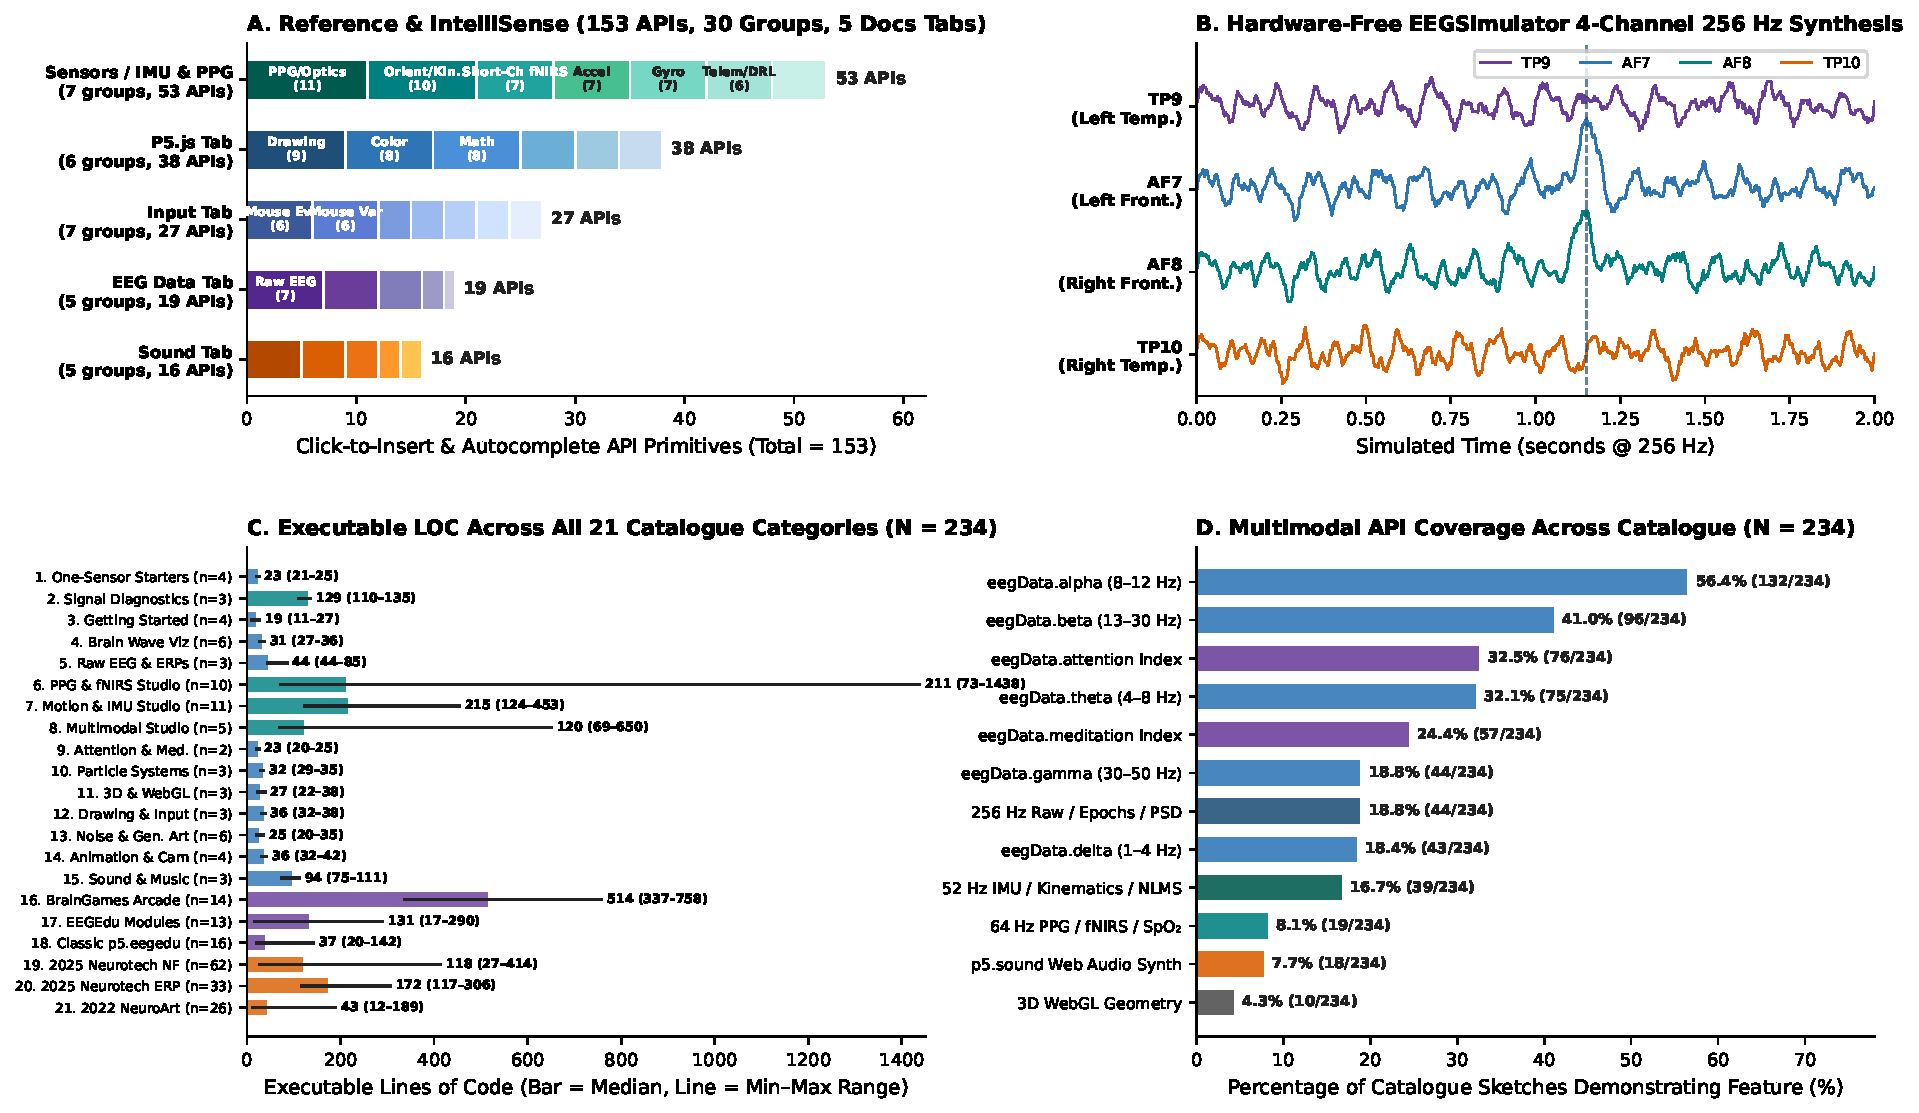
\includegraphics[width=0.98\textwidth]{figures/fig2_ide_scaffolding_and_corpus.pdf}
\caption{\textbf{Classroom Coding Supports, Hardware-Free Simulation, and \NCatalogueCategories-Category Visual Catalogue Profile ($N = \NCatalogueSketches$ Sketches).} \textbf{(A)} Distribution of the \NRefAPIs\ click-to-insert API entries across \NRefGroups\ groups and \NRefTabs\ reference tabs (\emph{Sensors / IMU \& PPG}: \NRefSensors; \emph{P5.js}: \NRefPFive; \emph{Input}: \NRefInput; \emph{EEG Data}: \NRefEEGData; \emph{Sound}: \NRefSound). \textbf{(B)} Two-second 4-channel simulated 256~Hz EEG traces showing ongoing oscillations and synchronous frontal eye blinks (\texttt{TP9}, \texttt{AF7}, \texttt{AF8}, \texttt{TP10} in \texttt{EEGSimulator}). \textbf{(C)} Executable lines of code across the \NCatalogueCategories\ categories in the Visual Catalogue ($N = \NCatalogueSketches$ sketches, overall $\text{median} = \CatLOCMedian\text{ LOC}$, range $\CatLOCMin\text{--}\CatLOCMax\text{ LOC}$; bars show category median and lines span min--max range). \textbf{(D)} Percentage of the \NCatalogueSketches\ catalogue sketches demonstrating each sensor and multimedia capability: alpha ($\CatPctAlpha\%$, $\CatCntAlpha/\NCatalogueSketches$), beta ($\CatPctBeta\%$, $\CatCntBeta/\NCatalogueSketches$), attention ($\CatPctAtt\%$, $\CatCntAtt/\NCatalogueSketches$), theta ($\CatPctTheta\%$, $\CatCntTheta/\NCatalogueSketches$), 256~Hz raw/ERP buffers ($\CatPctRaw\%$, $\CatCntRaw/\NCatalogueSketches$), 52~Hz IMU motion ($\CatPctIMU\%$, $\CatCntIMU/\NCatalogueSketches$), 64~Hz optical PPG/fNIRS ($\CatPctPPG\%$, $\CatCntPPG/\NCatalogueSketches$), and Web Audio synthesis ($\CatPctAudio\%$, $\CatCntAudio/\NCatalogueSketches$).}
\label{fig:scaffolding}
\end{figure}

\section{IDE Supports \& Visual Catalogue}

\subsection{Autocomplete \& Reference Drawer}

\subsubsection{Autocomplete \& Snippet Insertion}
Because most undergraduate neuroscience, psychology, and media-arts students enter the course with little or no programming background, the BrainImation editor includes several built-in supports designed to prevent syntax errors and lower coding anxiety \citep{iemi2026icancode} (Figure~\ref{fig:scaffolding}A). The left pane embeds the VS Code Monaco editor configured with custom autocomplete: as soon as a student types the shared signal object prefix, a pop-up menu lists the available brain, optical, and motion properties along with plain-English descriptions (\texttt{eegData.*}). Alongside the code editor, a collapsible right-hand Reference Drawer organizes \NRefAPIs\ functions and variables across \NRefTabs\ topic tabs covering optical and motion sensors, 2D and 3D drawing functions, keyboard and mouse controls, EEG band and ERP buffer properties, and Web Audio synthesis tools, plus an AI tutor tab that any student can open by pasting their own API key to receive guided coding explanations \citep{clindeffarges2026socrates} (Figure~\ref{fig:scaffolding}A). Clicking any entry in the Reference Drawer displays a short explanation of what the function does, and clicking it a second time inserts a ready-to-edit code snippet directly into the student's program at the cursor.

\subsubsection{Audio Unlock \& Link Sharing}
To streamline classroom troubleshooting and assignment grading, the top toolbar also includes an audio test button that plays a 1-second 440~Hz tone to unlock browser audio permissions, a quick-start guide, mobile fullscreen controls, and shareable web links that open a specific sketch automatically (\texttt{?sketch=}). Whenever a student clicks Run, the editor resets the graphics canvas and binds all drawing and audio functions automatically so standard introductory creative-coding tutorials work without extra boilerplate (\texttt{p5.js}, \texttt{p5.sound}).

\subsection{234-Sketch Visual Catalogue}

\subsubsection{Starters \& Core Scaffolds}
Rather than asking students or instructors to write code from a blank page, BrainImation provides a searchable Visual Catalogue containing \NCatalogueSketches\ runnable sketches across \NCatalogueCategories\ categories, each previewed with a visual thumbnail card (Figure~\ref{fig:ide}B,C and Figure~\ref{fig:scaffolding}C,D; $\text{median} = \CatLOCMedian\text{ LOC}$, range $\CatLOCMin\text{--}\CatLOCMax\text{ LOC}$). The \NCatalogueCategories\ categories are organized into six progressive learning tracks that guide users from short single-sensor examples to complete multimodal experiments and past student projects.

The first track pairs brief one-sensor starters and hardware check scripts with core creative-coding templates across ten foundational topics: getting started, brain wave visualizations, attention and meditation, particle systems, 3D geometry, interactive drawing, raw EEG waves, generative patterns, webcam motion, and sound synthesis (starters/diagnostics: $N = \NStarterDiag$, $\text{median} = \StarterDiagLOCMedian\text{ LOC}$, range $\StarterDiagLOCMin\text{--}\StarterDiagLOCMax\text{ LOC}$; core scaffolds: $N = \NBuiltinExamples$, $\text{median} = \ExLOCMedian\text{ LOC}$, range $\ExLOCMin\text{--}\ExLOCMax\text{ LOC}$). Students can open a 20--35 line template, see immediately how a single EEG rhythm changes screen color, particle speed, 3D rotation, or webcam effects, and begin experimenting by changing a few numbers.

\subsubsection{Optical, Motion, \& Heart Studios}
The second track, the optical PPG and fNIRS studio, introduces forehead pulse and prefrontal blood-oxygen sensing through step-by-step visual lessons \citep{wyser2020short,russo2025fnirs} ($N = \NPPGSketches$, $\text{median} = \StudioPPGLOCMedian\text{ LOC}$). Sequential sketches progress from a simple heartbeat pulse ring and raw red/infrared light traces to oxygenated and deoxygenated hemoglobin curves, a visual walkthrough of the Modified Beer--Lambert Law (comparing $660\text{ nm}/850\text{ nm}$ on Classic Muse with $730\text{ nm}/850\text{ nm}$ on Muse~S Athena, where $730\text{ nm}$ penetrates adult forehead tissue more effectively than $660\text{ nm}$ across the $20\text{ mm}$ spacing), an interactive 3D headband diagram comparing sensor layouts across headset generations, shallow ($8\text{ mm}$) versus deeper ($20\text{ mm}$) skin-pulse subtraction, and heart- or breath-paced biofeedback games.

The third track, the motion and diagnostics studio, applies the same step-by-step approach to the headband's 6-axis motion and status sensors \citep{rosanne2021adaptive,klug2022bemobil} ($N = \NIMUSketches$, $\text{median} = \StudioIMULOCMedian\text{ LOC}$). Individual lessons introduce the 3-axis accelerometer tilt meter, 3-axis gyroscope turn-rate display, 3D head pitch and roll horizon, battery and temperature gauges, and forehead electrode contact indicators, before showing how head acceleration integrates into velocity and 3D head position, how adaptive filtering subtracts head-movement artifacts from EEG, and how head tilt can steer musical instruments or 3D games.

The fourth track, the multimodal brain and heart studio, helps students compare physiological signals that unfold across three very different time scales \citep{makowski2021neurokit2,cannard2024brainbeats} ($N = \NMultiSketches$, $\text{median} = \StudioMultiLOCMedian\text{ LOC}$): fast millisecond event-related EEG potentials ($50\text{--}800\text{ ms}$), second-by-second fluctuations in oscillatory EEG band power and beat-to-beat heart rate ($0.5\text{--}2\text{ s}$), and the slower $4\text{--}6\text{ s}$ rise and fall of prefrontal blood oxygenation ($\Delta[\text{HbO}_2]$ and $\Delta[\text{HHb}]$). In particular, the Heartbeat-Evoked Potential (HEP) lesson time-locks 256~Hz EEG epochs to the participant's own heartbeat peak detected by the forehead optical sensor rather than an external screen flash \citep{cannard2024brainbeats,steinfath2025validating}, providing an intuitive classroom demonstration of brain--heart interoception, internal event-locked averaging, and the pulse travel time from ventricular contraction in the heart to the forehead vasculature ($\sim 150\text{--}250\text{ ms}$ transit delay with $\sim 10\text{--}25\text{ ms}$ beat-to-beat variability).

\subsubsection{BrainGames \& Lab Modules}
The fifth track shows how these signal-processing building blocks come together inside complete interactive applications through closed-loop neurofeedback arcade games and ready-to-run laboratory modules ($N = \NGamesAndEEGEdu$ sketches total). The arcade collection includes \NBrainGames\ playable games (such as \emph{Golf Driving Range}, \emph{Archery Range}, \emph{Rowing Calm}, \emph{Balance Beam}, and \emph{Zen Breakout}) built on a shared smoothing and scoreboard engine ($\text{median} = \BrainGamesLOCMedian\text{ LOC}$; \texttt{window.BGShared}), paired with \NEEGEduModules\ interactive curriculum lessons and \NClassicEEGEdu\ classic laboratory ports covering standard neuroscience paradigms such as oddball ERPs and steady-state visual evoked potentials with CSV spreadsheet export.

\subsubsection{Archival Student Galleries}
The sixth track preserves two archival classroom galleries of playable student projects ($N = \NArchivalTotal$ total: \NNeurotechCatalogue\ submissions from the 2025 Neurotech cohort, $\text{median} = \NeurotechLOCMedian\text{ LOC}$; \NNeuroArtGallery\ projects from the 2022 NeuroArt cohort, $\text{median} = \NeuroArtLOCMedian\text{ LOC}$). Including past student work directly inside the Visual Catalogue gives incoming students concrete, runnable examples of what peers with similar neuroscience and psychology backgrounds created in a single semester. Across all \NCatalogueSketches\ catalogue sketches, continuous EEG band powers and attention/meditation indices are the most commonly used signals, followed by raw 256~Hz ERP buffers, 6-axis head motion, optical PPG/fNIRS blood-flow metrics, and Web Audio synthesis (Figure~\ref{fig:scaffolding}D).

\begin{figure}[t!]
\centering
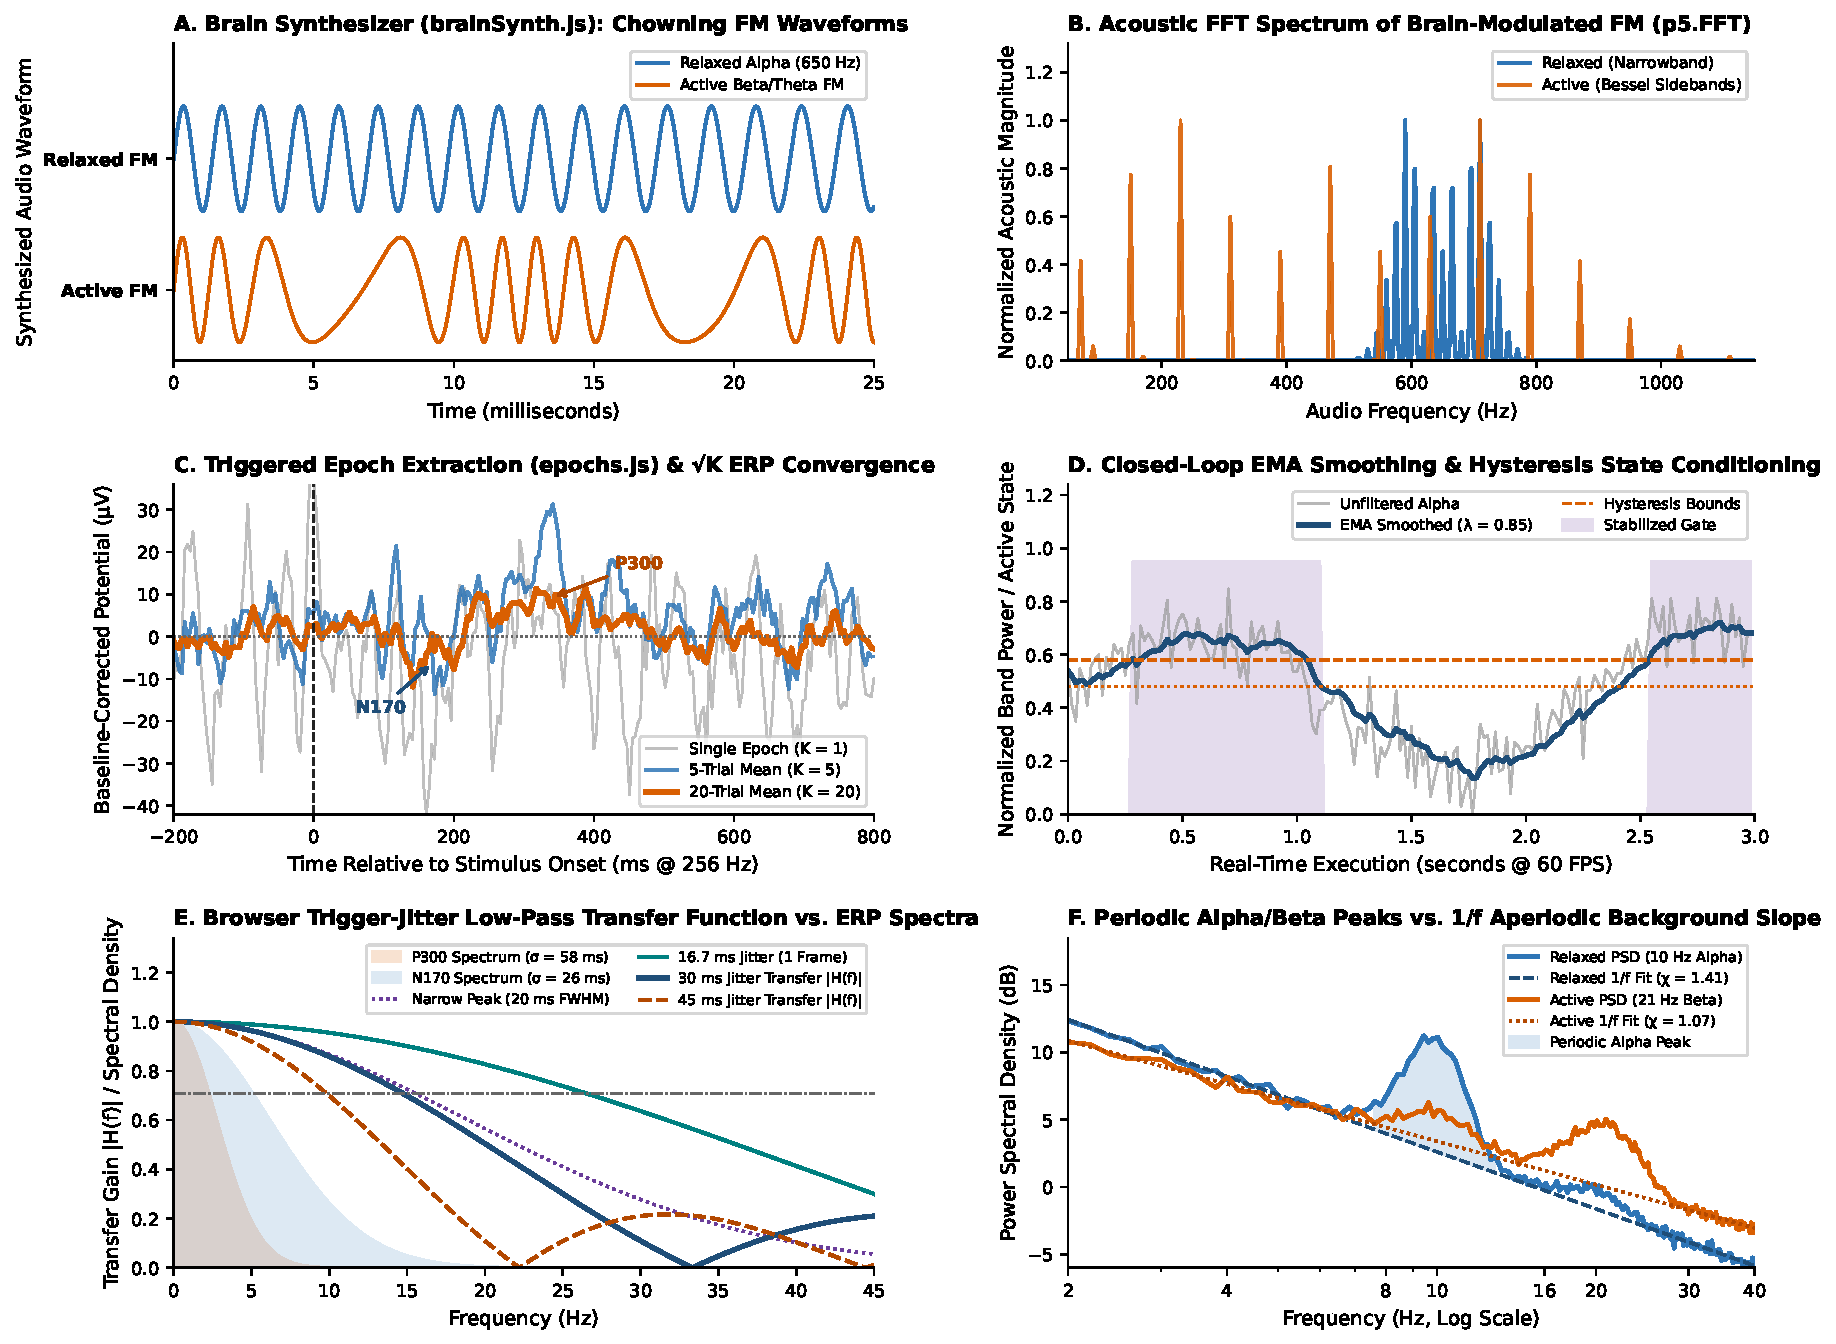
\includegraphics[width=0.98\textwidth]{figures/fig3_sonification_and_erp_engine.pdf}
\caption{\textbf{Teaching Modules for Audio Sonification, Online 4-Channel ERP Averaging, Frame-Jitter Transfer, and Periodic/Aperiodic Spectra.} \textbf{(A)} Audio waveforms comparing a relaxed high-alpha state ($650\text{ Hz}$ smooth tone) against an active high-beta/theta state (\texttt{brainSynth.js}). \textbf{(B)} Corresponding audio frequency spectra showing a single dominant frequency during relaxation versus harmonic sidebands during active engagement (\texttt{p5.FFT}). \textbf{(C)} Online 256~Hz ERP trial averaging ($-200\text{ to }+800\text{ ms}$, positive-up voltage convention in $\mu\text{V}$, baseline-corrected over $-200\text{ to }0\text{ ms}$; \citealp{picton2000guidelines,keil2014committee}) across $K = 1, 5,$ and $20$ trials (\texttt{epochs.js}). Across 1,000 Monte Carlo runs, pre-stimulus baseline RMS noise scales by $1/\sqrt{K}$ ($\ERPMCNoiseRMSKOne \rightarrow \ERPMCNoiseRMSKFive \rightarrow \ERPMCNoiseRMSKTwenty\ \mu\text{V}$); in the single realization shown, baseline RMS drops from $\ERPNoiseRMSKOne\ \mu\text{V}$ ($\text{SNR} = \ERPSNRKOne$) to $\ERPNoiseRMSKFive\ \mu\text{V}$ ($\text{SNR} = \ERPSNRKFive$) and $\ERPNoiseRMSKTwenty\ \mu\text{V}$ ($\text{SNR} = \ERPSNRKTwenty$), while P300 Standardized Measurement Error ($\text{SME} = \text{SD}_{\text{trials}}/\sqrt{K}$; \citealp{luck2021standardized}) drops from $\ERPSMEKOne \rightarrow \ERPSMEKFive \rightarrow \ERPSMEKTwenty\ \mu\text{V}$. Rejecting a single $115\ \mu\text{V}$ blink trial ($\ERPBlinkPtPUV\ \mu\text{V}$ peak-to-peak) eliminates $+\ERPBlinkPThreeHundredBiasUV\ \mu\text{V}$ of P300 peak bias ($\text{RMSE}: \ERPRMSEBlinkUnrejectedUV \rightarrow \ERPRMSEBlinkRejectedUV\ \mu\text{V}$, vs.\ $\ERPRMSECleanTwentyUV\ \mu\text{V}$ blink-free). \textbf{(D)} Exponential moving-average smoothing and dual-threshold hysteresis used in student neurofeedback games to prevent rapid on/off flicker ($\EMAVarReductionPct\%$ jitter variance reduction). \textbf{(E)} Frequency-domain $\text{sinc}$ transfer function $|H(f)| = |\text{sinc}(fW)|$ for browser/Bluetooth trigger jitter of $W = 16.7\text{ ms}$ (1 frame @ 60~FPS, $f_c = \JitterFCMSixteenHz\text{ Hz}$), $30\text{ ms}$ ($f_c = \JitterFCThirtyHz\text{ Hz}$, null at $\JitterNullThirtyHz\text{ Hz}$), and $45\text{ ms}$ ($f_c = \JitterFCFortyFiveHz\text{ Hz}$, null at $\JitterNullFortyFiveHz\text{ Hz}$) overlaid on normalized spectral profiles of the P300 ($\sigma = 58\text{ ms}$), N170 ($\sigma = 26\text{ ms}$), and a narrow $20\text{ ms}$ FWHM peak; across 1,000 20-trial runs under $30\text{ ms}$ jitter, P300 latency SD drops from $\JitterPThreePeakLatSDMS\text{ ms}$ (peak picking) to $\JitterPThreeTempLatSDMS\text{ ms}$ (dynamic template matching; \citealp{schubert2026dynamic}) and $\JitterPThreeAreaLatSDMS\text{ ms}$ (50\% fractional-area latency; \citealp{schubert2024multiverse}). \textbf{(F)} Log-log power spectral density ($2\text{--}40\text{ Hz}$) separating periodic $10\text{ Hz}$ alpha ($+\AlphaPeakAboveOneFRelDB\text{ dB}$ vs.\ $+\AlphaPeakAboveOneFActDB\text{ dB}$ above the $1/f^{\chi}$ background; $\Delta = \AlphaAdjDiffDB\text{ dB}$ vs.\ $\AlphaRawDiffDB\text{ dB}$ unadjusted) from the aperiodic $1/f^{\chi}$ exponent ($\chi = \AperiodicExpRelaxed$ relaxed vs.\ $\AperiodicExpActive$ active; \citealp{vanbueren2026comparing}).}
\label{fig:sonification}
\end{figure}

\section{Core Teaching Modules}

\subsection{Audio Sonification}

\subsubsection{EEG-to-FM Parameter Mapping}
Turning continuous brain activity into sound (sonification) is especially valuable in neuroscience and psychology labs that study eyes-closed relaxation, mindfulness, emotion-driven musical feedback, or interactive human--AI performance loops, where asking a participant to watch a computer screen would interfere with the state being measured \citep{livingstone2018ravdess,takabatake2021musical,livingstone2026music,monroydcroz2026minimalist} (Figure~\ref{fig:sonification}A,B). After starting with simple pitch mapping and musical scale notes (\texttt{brainBeats.js}, \texttt{alphaMusic.js}), students can open the frequency-modulation (FM) synthesizer lesson to see how four EEG rhythms simultaneously shape a continuous musical tone \citep{chowning1973synthesis} (\texttt{brainSynth.js}). In FM synthesis, one oscillator generates the main musical pitch (the carrier) while a second oscillator (the modulator) rapidly vibrates that pitch to create harmonic overtones. In the sketch code below, alpha power controls the main pitch, beta power controls how fast the modulator vibrates, theta power controls how strongly the modulator adds overtones (timbre complexity), and the attention index smoothly adjusts the overall volume:

\noindent\begin{minipage}{\textwidth}
\begin{lstlisting}
// Core FM synthesis mapping from examples/brainSynth.js
let carrierFreq = map(eegData.alpha, 0, 1, 200, 800); // Alpha -> pitch (200-800 Hz)
let modFreq     = map(eegData.beta,  0, 1, 0, 100);   // Beta  -> modulation rate
let modDepth    = map(eegData.theta, 0, 1, 0, 500);   // Theta -> harmonic depth
let volume      = map(eegData.attention, 0, 1, 0, 0.2);

carrier.freq(carrierFreq);
modulator.freq(modFreq);
modulator.amp(modDepth);
carrier.amp(volume, 0.1); // 100 ms ramp prevents audio clicks between frames
\end{lstlisting}
\end{minipage}
\vspace{4pt}

\subsubsection{Relaxed vs.\ Engaged Spectra}
As illustrated in Figure~\ref{fig:sonification}A,B, when a participant relaxes with eyes closed (high alpha power, low beta and theta power; \citealp{takabatake2021musical}), the synthesizer produces a pure, flute-like $650\text{ Hz}$ sine wave with a single peak in the frequency spectrum. When beta and theta power rise during active mental engagement, the modulator introduces sideband frequencies on either side of the main pitch, creating a richer harmonic texture that students can both hear through their headphones and observe on the live spectrum display \citep{livingstone2018ravdess,monroydcroz2026minimalist}.

\subsubsection{Periodic vs.\ Aperiodic Spectra}
When teaching spectral neurofeedback on consumer-grade and classroom EEG headbands, recent methodological investigations highlight an important distinction between narrowband periodic oscillations (such as the $8\text{--}12\text{ Hz}$ alpha peak) and the underlying broadband $1/f^{\chi}$ aperiodic background spectrum, whose power decays with frequency according to $\log_{10} P(f) = b - \chi \log_{10} f$ \citep{cannard2021validating,sabio2024scoping,vanbueren2026comparing,dekleijn2023short}. In a recent comparison of consumer-grade and research-grade EEG systems, \citet{vanbueren2026comparing} demonstrated that shifts in the aperiodic exponent ($\chi$) and offset ($b$) carry distinct neurocognitive and developmental information and can confound raw band-power ratios if students mistake a broadband tilt of the $1/f^{\chi}$ background for a change in true oscillatory alpha power. To help instructors illustrate this concept, Figure~\ref{fig:sonification}F plots the log-log power spectral density ($2\text{--}40\text{ Hz}$) across relaxed eyes-closed and active engaged states alongside the linear least-squares fit of the $1/f^{\chi}$ background across non-oscillatory anchor frequencies ($2\text{--}6\text{ Hz}$ and $30\text{--}40\text{ Hz}$). Separating the aperiodic background slope ($\chi = \AperiodicExpRelaxed$ relaxed vs.\ $\AperiodicExpActive$ active) from the narrowband $10\text{ Hz}$ alpha bump reveals that periodic alpha power rises $+\AlphaPeakAboveOneFRelDB\text{ dB}$ above the $1/f^{\chi}$ line during eyes-closed relaxation versus $+\AlphaPeakAboveOneFActDB\text{ dB}$ during active engagement ($\Delta = \AlphaAdjDiffDB\text{ dB}$ aperiodic-adjusted vs.\ $\AlphaRawDiffDB\text{ dB}$ unadjusted), giving students a transparent visual bridge between simple classroom band-power bars and modern parameterized spectral analysis \citep{cannard2021validating,vanbueren2026comparing}.

\subsection{Online ERP Averaging}

\subsubsection{Forehead Reference \& Polarity}
In cognitive neuroscience and experimental psychology courses, event-related potentials (ERPs) teach students how time-locked averaging extracts small sensory and cognitive brain responses (typically $2\text{--}10\ \mu\text{V}$) from ongoing background EEG waves that are several times larger, providing neural chronometry measures that can be linked to behavioral response times and cognitive models \citep{luck2014introduction,krigolson2017choosing,frischkorn2018cognitive,schubert2023enhancing,nunez2024tutorial} (Figure~\ref{fig:sonification}C; \texttt{epochs.js}). When introducing ERPs on a portable headband, an important concept for instructors to explain is the location of the reference electrode. Traditional laboratory EEG caps place their reference electrode on the earlobe or mastoid bone behind the ear, whereas the Muse headband places its reference and ground electrodes on the center of the forehead (\texttt{REF}/\texttt{DRL} at \texttt{Fpz}). Because every EEG channel measures the voltage difference between the recording electrode and the reference site, recording from the behind-the-ear sensors against an active forehead reference ($V_{\text{TP9/TP10}} - V_{\text{Fpz}}$) reverses the upward/downward direction of classic parietal or vertex oddball waves unless students re-reference the behind-the-ear channels against the forehead channels ($V_{\text{TP}} - V_{\text{AF}}$; \citealp{krigolson2017choosing}) or flip the sign in code. To avoid confusing beginners when they first learn how ERP waves look, our built-in signal simulator injects the familiar textbook polarities directly into the left temporal channel (e.g., a negative-going N170 peak ($-6.5\ \mu\text{V}$) followed by a positive-going P300 peak ($+9.5\ \mu\text{V}$)) so students can first master trial averaging and component identification before exploring reference montages on live headbands (Figure~\ref{fig:sonification}C; \texttt{TP9} in \texttt{EEGSimulator}).

\subsubsection{Epoch Extraction \& Large Amplitude Rejection}
Every $1.5\text{ s}$ (90 animation frames), the ERP teaching template flashes a visual stimulus on screen. It then waits 48 frames ($+800\text{ ms}$) so the full post-stimulus brain response has been recorded into the 256~Hz buffer, extracts a 1-second window of data (256 samples spanning $-200\text{ ms}$ before the flash to $+800\text{ ms}$ after the flash), subtracts the average voltage during the $-200\text{ to }0\text{ ms}$ pre-stimulus baseline so every trial starts aligned at $0\ \mu\text{V}$, rejects any trial containing a large $>100\ \mu\text{V}$ amplitude spike, and folds the clean trial into a running average across all four electrodes:

\noindent\begin{minipage}{\textwidth}
\begin{lstlisting}
// Online ERP epoch extraction, blink rejection, and baseline correction (examples/epochs.js)
if (waitingForEpoch && frameCount >= stimulusFrame + 48) { // +800 ms post-stimulus
  let rawEpoch = eegData.getRecentEpoch(256); // 256 samples (1000 ms @ 256 Hz) x 4 channels
  let baselineSamples = 51;                   // First 51 samples = -200 ms to 0 ms baseline
  let hasBlink = false, baseMean = [0, 0, 0, 0];
  for (let ch = 0; ch < 4; ch++) {
    let minV = Infinity, maxV = -Infinity;
    for (let s = 0; s < 256; s++) {
      if (s < baselineSamples) baseMean[ch] += rawEpoch[s][ch] / baselineSamples;
      if (rawEpoch[s][ch] < minV) minV = rawEpoch[s][ch];
      if (rawEpoch[s][ch] > maxV) maxV = rawEpoch[s][ch];
    }
    if (maxV - minV > 100) hasBlink = true;   // >100 uV peak-to-peak whole-epoch rejection
  }
  if (!hasBlink) {                            // Update running average only on clean epochs
    trialCount++;
    for (let ch = 0; ch < 4; ch++) {
      for (let s = 0; s < 256; s++) {
        let corrected = rawEpoch[s][ch] - baseMean[ch];
        avgERP[s][ch] = ((avgERP[s][ch] * (trialCount - 1)) + corrected) / trialCount;
      }
    }
  }
  waitingForEpoch = false;
}
\end{lstlisting}
\end{minipage}
\vspace{4pt}

\subsubsection{$\sqrt{K}$ Scaling, SME, \& Hysteresis}
Because ongoing background EEG oscillations are not locked to the timing of the visual flash, averaging $K$ independent trials cancels out background noise in proportion to the square root of the trial count ($\sqrt{K}$). Over 20 trials, this noise reduction lowers the trial-to-trial Standardized Measurement Error (SME) by more than fourfold and allows the N170 and P300 peaks to stand out clearly from the background EEG ($1/\sqrt{K}$ scaling: $\text{RMS} = \ERPNoiseRMSKOne \rightarrow \ERPNoiseRMSKTwenty\ \mu\text{V}$, $\text{SNR} = \ERPSNRKOne \rightarrow \ERPSNRKTwenty$, P300 $\text{SME} = \ERPSMEKOne \rightarrow \ERPSMEKTwenty\ \mu\text{V}$; \citealp{luck2021standardized,schubert2023enhancing}; see Figure~\ref{fig:sonification}C caption for Monte Carlo benchmarks). This large amplitude rejection rule teaches an equally important practical lesson. For example, an eye blink is one such spike: because a single eye blink generates a voltage spike more than ten times larger than an ERP peak, leaving just one blink trial inside a 20-trial average severely distorts the P300 wave, whereas rejecting that single contaminated trial restores the true waveform ($\text{RMSE}: \ERPRMSEBlinkUnrejectedUV \rightarrow \ERPRMSEBlinkRejectedUV\ \mu\text{V}$; Figure~\ref{fig:sonification}C). For continuous neurofeedback games, students also learn two simple techniques to keep on-screen control smooth and responsive: blending each new frame of band power with the previous value (an exponential moving average) to calm rapid moment-to-moment fluctuations, and using separate turn-on and turn-off thresholds (hysteresis, much like a home thermostat) so game states do not flicker rapidly when a player's brain state hovers near the threshold ($\EMAVarReductionPct\%$ jitter variance reduction; \texttt{smoothAlpha = 0.85 * smoothAlpha + 0.15 * eegData.alpha}; Figure~\ref{fig:sonification}D).

\subsubsection{Frame Jitter \& Latency}
A central methodological question in browser-based chronometry and portable EEG is how display frame intervals and Bluetooth packet arrival jitter affect ERP component amplitudes and latencies \citep{pronk2020mental,anwyl2021realistic,lukacs2023precise,schubert2024multiverse,schubert2026dynamic}. Large-scale timing benchmarks across web browsers and operating systems show that standard requestAnimationFrame display loops achieve sub-frame precision when properly synchronized \citep{pronk2020mental,lukacs2023precise}, whereas combined browser rendering and wireless packet buffering introduce $\sim 15\text{--}45\text{ ms}$ of trial-to-trial trigger jitter when hardware photodiode triggers are absent \citep{anwyl2021realistic,krigolson2017choosing}. Mathematically, convolving an ERP waveform with a uniform trigger-jitter window of width $W$ multiplies its frequency spectrum by the low-pass transfer function $|H(f)| = |\text{sinc}(fW)|$. As shown in Figure~\ref{fig:sonification}E, a 1-frame ($16.7\text{ ms}$), $30\text{ ms}$, or $45\text{ ms}$ jitter window imposes $-3\text{ dB}$ half-power cutoffs at $\JitterFCMSixteenHz\text{ Hz}$, $\JitterFCThirtyHz\text{ Hz}$, and $\JitterFCFortyFiveHz\text{ Hz}$, respectively: while $30\text{ ms}$ jitter attenuates a narrow $20\text{ ms}$ sensory spike to $\JitterRetNarrowPct\%$ of its true peak, the broader spectral envelopes of the N170 ($\sigma = 26\text{ ms}$, concentrated below $10\text{ Hz}$) and P300 ($\sigma = 58\text{ ms}$, concentrated below $5\text{ Hz}$) retain $\JitterRetNOneSeventyPct\%$ and $\JitterRetPThreeHundredPct\%$ of their peak amplitude. Furthermore, when extracting P300 latency from noisy 20-trial classroom averages under $30\text{ ms}$ trigger jitter across 1,000 Monte Carlo runs, our benchmark directly confirms the multiverse and dynamic template-matching findings of \citet{schubert2024multiverse} and \citet{schubert2026dynamic}: whereas naive maximum-peak picking suffers substantial latency variability from residual high-frequency noise ($\text{SD} = \JitterPThreePeakLatSDMS\text{ ms}$), dynamic Gaussian template matching ($\text{SD} = \JitterPThreeTempLatSDMS\text{ ms}$; \citealp{schubert2026dynamic}) and 50\% positive fractional-area latency ($\text{SD} = \JitterPThreeAreaLatSDMS\text{ ms}$; \citealp{schubert2024multiverse}) improve P300 latency precision by nearly threefold.

\begin{figure}[t!]
\centering
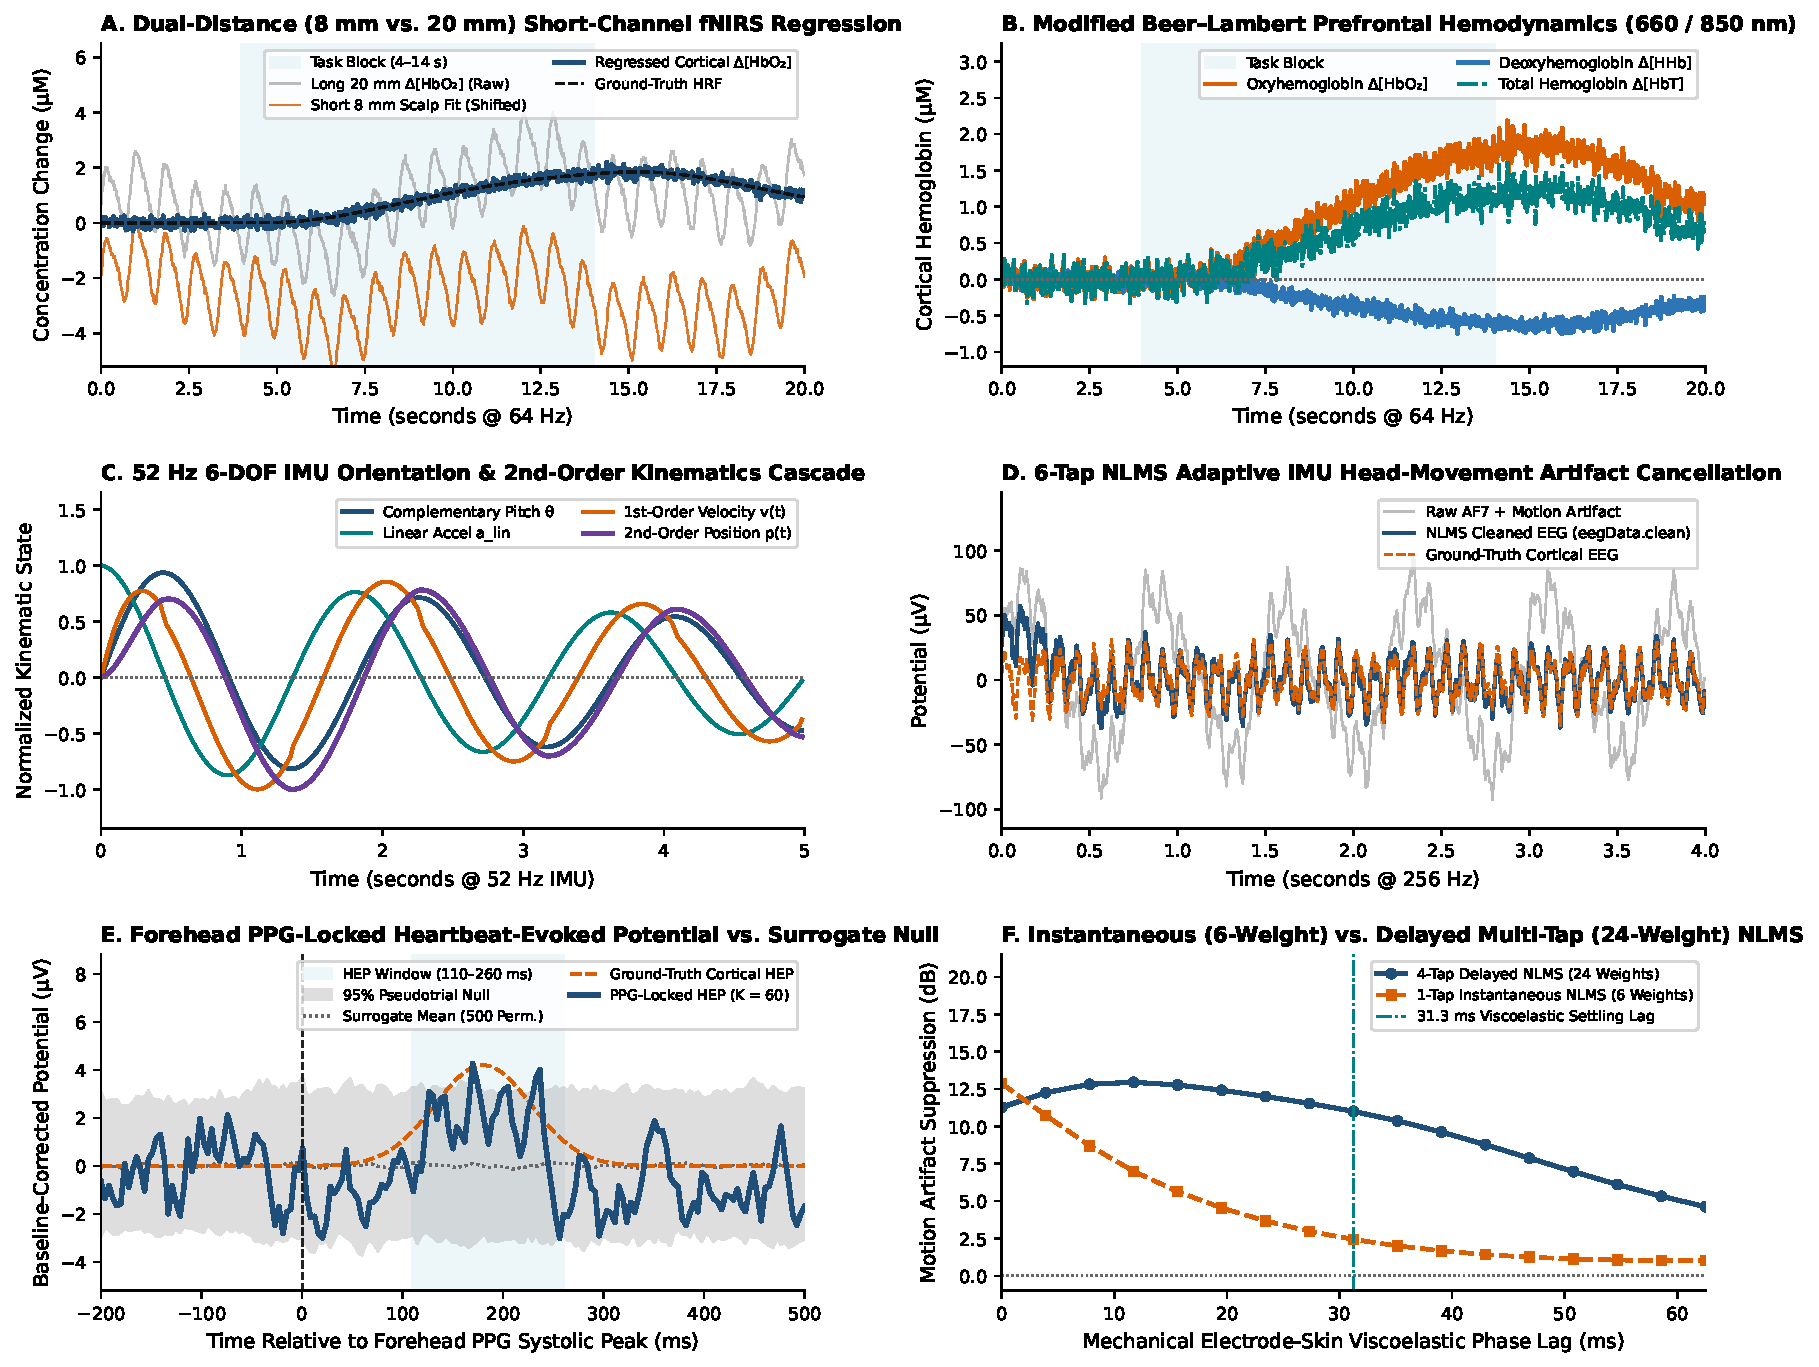
\includegraphics[width=0.98\textwidth]{figures/fig4_multimodal_athena_ppg_imu.pdf}
\caption{\textbf{Teaching Modules for Optical fNIRS Short-Channel Skin Regression, Heartbeat-Evoked Potentials, and 6-DOF IMU Motion Filtering.} \textbf{(A)} Simulated dual-distance ($8\text{ mm}$ short channel vs.\ $20\text{ mm}$ long channel) optical blood-flow traces, showing how subtracting the scaled $8\text{ mm}$ superficial skin signal removes heart-pulse ($1.18\text{ Hz}$), breathing ($0.26\text{ Hz}$), and Mayer-wave ($0.10\text{ Hz}$) contamination ($\FNIRSSuppDB\text{ dB}$ reduction; $\text{RMSE}: \FNIRSErrRawUM \rightarrow \FNIRSErrCleanUM\ \mu\text{M}$ [$\FNIRSErrRawUMThreeD \rightarrow \FNIRSErrCleanUMThreeD\ \mu\text{M}$ unrounded], $r: \FNIRSRRaw \rightarrow \FNIRSRClean$; \citealp{wyser2020short,russo2025fnirs}). \textbf{(B)} Resulting prefrontal oxyhemoglobin ($\Delta[\text{HbO}_2]$), deoxyhemoglobin ($\Delta[\text{HHb}]$), and total hemoglobin ($\Delta[\text{HbT}]$) response during a simulated task block ($4\text{--}14\text{ s}$). \textbf{(C)} 52~Hz 6-DOF IMU head tilt angle (\texttt{pitch}, peak $\pm 16^{\circ}$), gravity-removed linear acceleration (peak $\pm 1.4\text{ m/s}^2$), 1st-order head velocity ($\text{cm/s}$), and 2nd-order 3D head displacement ($\text{cm}$), each normalized to unit peak amplitude ($[-1, 1]$) for joint comparison. \textbf{(D)} Adaptive 6-tap NLMS filtering of simulated head-movement artifacts on frontal EEG (\texttt{AF7}), reducing synchronous motion artifact by $\NLMSSuppDB\text{ dB}$ ($\text{RMSE}: \NLMSRMSERawUV \rightarrow \NLMSRMSECleanUV\ \mu\text{V}$, $r: \NLMSRRaw \rightarrow \NLMSRClean$). \textbf{(E)} Forehead PPG-locked Heartbeat-Evoked Potential ($K = 60$ beats, $\sim 180\text{ ms}$ pulse transit delay with $\sigma_{\text{PTT}} = 12\text{ ms}$ jitter; peak $\HEPTruePeakUV\ \mu\text{V}$, window mean $\HEPTrueWinMeanUV\ \mu\text{V}$, $\text{SME} = \HEPSMEUV\ \mu\text{V}$) compared against a 500-permutation surrogate pseudotrial null distribution (95\% null band $\pm \HEPSurrCIUV\ \mu\text{V}$, permutation $p = \HEPPermP$; \citealp{cannard2024brainbeats,steinfath2025validating}). \textbf{(F)} Motion artifact suppression across mechanical electrode-skin viscoelastic phase lags ($\tau_{\text{lag}} = 0\text{--}62.5\text{ ms}$), comparing the instantaneous 1-tap-per-axis (6-weight) NLMS filter against a 4-tap-per-axis (24-weight) delayed FIR NLMS filter ($\NLMSLagThirtyOneFourTapDB\text{ dB}$ vs.\ $\NLMSLagThirtyOneOneTapDB\text{ dB}$ at $\tau_{\text{lag}} = 31.3\text{ ms}$, $+\NLMSLagThirtyOneGainDB\text{ dB}$ gain; \citealp{rosanne2021adaptive,klug2022bemobil}).}
\label{fig:multimodal}
\end{figure}

\subsection{Optical PPG/fNIRS Regression}

\subsubsection{Beer--Lambert Contrast \& Depth}
Whereas EEG measures fast electrical activity in milliseconds, functional near-infrared spectroscopy (fNIRS) teaches students how optical sensors measure the slower hemodynamic response: a local rise in oxygenated hemoglobin ($\text{HbO}_2$) and a dip in deoxygenated hemoglobin ($\text{HHb}$), peaking $4\text{--}6\text{ s}$ after a brain region becomes active. This is the same neurovascular coupling, as measured by functional MRI, and used to track prefrontal cognitive load \citep{delpy1988estimation,scholkmann2014review,russo2025fnirs}. To separate oxygenated from deoxygenated blood, the headband shines two wavelengths of light located on opposite sides of $800\text{ nm}$, the crossover point where both forms of hemoglobin absorb light equally: below $800\text{ nm}$ (Red $660\text{ nm}$ on Classic Muse, or Near-Infrared $730\text{ nm}$ on Muse~S Athena, which passes through adult forehead tissue more easily than $660\text{ nm}$), deoxygenated blood absorbs more light, whereas at $850\text{ nm}$ (Infrared), oxygenated blood absorbs more light. Comparing the returning light at both wavelengths allows the software to calculate relative concentration changes via the Modified Beer--Lambert Law.

When light shines into the forehead, the scattered photons travel from the LED to the photodetector along a curved, banana-shaped path whose depth reaches roughly one-third to one-half of the distance between the light source and detector \citep{delpy1988estimation,saager2005direct,wyser2020short}. Consequently, a detector placed close to the LED ($8\text{ mm}$ short channel) reaches only $\sim 3\text{--}4\text{ mm}$ deep, measuring blood flow exclusively in the superficial scalp and forehead skin. By contrast, a detector placed farther from the LED ($20\text{ mm}$ long channel) reaches $\sim 7\text{--}10\text{ mm}$ deep, capturing signals that pass through both the overlying skin and the surface of the prefrontal cortex.

\subsubsection{Short-Channel Skin Regression}
Because the deeper $20\text{ mm}$ channel still passes through the scalp, its raw optical trace is heavily rhythmic with superficial skin activity, including the heartbeat pulse, breathing cycles, and slow blood-pressure waves (Mayer waves around $0.1\text{ Hz}$; \citealp{scholkmann2014review,wyser2020short}). Because the Muse~S Athena headband (and our simulator) records both the $8\text{ mm}$ and $20\text{ mm}$ channels simultaneously, students can see how simple linear regression removes superficial skin noise to uncover the deeper cortical response:

\noindent\begin{minipage}{\textwidth}
\begin{lstlisting}
// Short-channel (8 mm) vs. Long-channel (20 mm) regression in updateShortChannelRegression()
// 1. Estimate scaling factor beta between short (skin) and long (skin + brain) optical density
let covSL = 0, varS = 0;
for (let k = 0; k < W; k++) {
  let ds = shortOD[k] - meanShort;
  let dl = longOD[k]  - meanLong;
  covSL += ds * dl;
  varS  += ds * ds;
}
let beta = covSL / (varS + 1e-6);

// 2. Subtract scaled skin signal from long channel, then convert to HbO2 and HHb
let cleanOD_Red = currentLongOD_Red - betaRed * currentShortOD_Red;
let cleanOD_IR  = currentLongOD_IR  - betaIR  * currentShortOD_IR;
\end{lstlisting}
\end{minipage}
\vspace{4pt}

As shown in Figure~\ref{fig:multimodal}A,B, subtracting the scaled $8\text{ mm}$ skin signal from the $20\text{ mm}$ long channel strips away the large heartbeat, breathing, and blood-pressure oscillations and clearly reveals the slow prefrontal rise in oxygenated hemoglobin and accompanying drop in deoxygenated hemoglobin during the cognitive task block ($\FNIRSSuppDB\text{ dB}$ superficial artifact suppression; $\text{RMSE}: \FNIRSErrRawUM \rightarrow \FNIRSErrCleanUM\ \mu\text{M}$, $r = \FNIRSRRaw \rightarrow \FNIRSRClean$; \citealp{wyser2020short,russo2025fnirs}).

\subsubsection{Heartbeat Potentials \& Surrogates}
Whereas short-channel fNIRS treats the forehead arterial pulse as superficial noise to be regressed out, brain--heart interoception research uses that same cardiac pulse as an endogenous physiological time-lock to extract Heartbeat-Evoked Potentials (HEPs) from the EEG \citep{makowski2021neurokit2,cannard2024brainbeats,steinfath2025validating}. On a wearable headband without chest ECG electrodes, 64~Hz forehead PPG systolic peaks provide a convenient non-invasive cardiac trigger that arrives $\sim 180\text{ ms}$ after the ventricular R-peak with modest beat-to-beat pulse-transit jitter ($\sigma_{\text{PTT}} \approx 12\text{ ms}$). A crucial methodological caveat in HEP research, recently formalized by \citet{steinfath2025validating}, is that ongoing low-frequency EEG fluctuations or cardiac field artifacts can masquerade as apparent heartbeat-locked deflections unless researchers test their observed waveform against a \emph{surrogate pseudotrial null distribution} constructed by randomly permuting the inter-beat intervals. As illustrated in Figure~\ref{fig:multimodal}E, averaging $K = 60$ forehead PPG-locked EEG epochs ($-200\text{ to }+500\text{ ms}$ relative to the systolic pulse peak, baseline-corrected over $-200\text{ to }-50\text{ ms}$) recovers a clear frontocentral HEP wave across the $+110\text{ to }+260\text{ ms}$ post-PPG window (corresponding to $+290\text{ to }+440\text{ ms}$ post-R-peak) that rises significantly above the 95\% surrogate pseudotrial null envelope generated from 500 random inter-beat interval permutations (peak $= \HEPTruePeakUV\ \mu\text{V}$, window mean $= \HEPTrueWinMeanUV\ \mu\text{V}$, $\text{SME} = \HEPSMEUV\ \mu\text{V}$, 95\% surrogate null band $= \pm \HEPSurrCIUV\ \mu\text{V}$, permutation $p = \HEPPermP$; \citealp{cannard2024brainbeats,steinfath2025validating}).

\subsection{Head Motion \& NLMS Filtering}

\subsubsection{6-DOF Kinematics Integration}
The motion studio sketches introduce two complementary uses for the headband's 52~Hz 3-axis accelerometer and 3-axis gyroscope \citep{rosanne2021adaptive,klug2022bemobil}. In the kinematics lesson (Figure~\ref{fig:multimodal}C), students see how combining accelerometer and gyroscope measurements tracks 3D head tilt angles (nodding pitch, side-to-side roll, and turning yaw), how subtracting the constant pull of gravity isolates true linear head acceleration, and how accumulating acceleration over time estimates head movement speed ($\text{cm/s}$) and 3D head displacement ($\text{cm}$).

\subsubsection{6-Tap NLMS Motion Filter}
In the adaptive motion-filtering lesson (Figure~\ref{fig:multimodal}D), students learn how those same 6-axis head-movement signals can clean up movement artifacts in the EEG trace \citep{widrow1975adaptive,rosanne2021adaptive,klug2022bemobil,mathewson2024moving}. Whenever a participant nods or tilts their head, slight mechanical shifts of the dry electrodes create large voltage swings that mirror the head motion. Because the headband measures 6-axis head motion at the same time as the EEG, an adaptive filter can continuously estimate how much of the current EEG voltage is predicted by the six motion axes, subtract that predicted movement artifact from each electrode, and gently update its six scaling weights on every sample:

\noindent\begin{minipage}{\textwidth}
\begin{lstlisting}
// 6-tap adaptive (NLMS) head-movement filter in updateEEGImuMotionFilter()
let u = [0.25*linAx, 0.25*linAy, 0.25*linAz, gx/80, gy/80, gz/80]; // 6-axis IMU reference
let normU = u.reduce((sum, v) => sum + v * v, 0) + 1e-4;

for (let ch = 0; ch < 4; ch++) {
  let w = eegData.motionFilterWeights[ch];
  let estArtifact = 0;
  for (let i = 0; i < 6; i++) estArtifact += w[i] * u[i];
  let cleanEEG = eegData.raw[ch] - estArtifact; // Subtract predicted motion artifact

  // Update filter weights slightly on each sample (mu = 0.035)
  for (let i = 0; i < 6; i++) {
    w[i] = 0.9992 * w[i] + (0.035 * cleanEEG * u[i]) / normU;
  }
  eegData.clean[ch] = cleanEEG;
}
\end{lstlisting}
\end{minipage}
\vspace{4pt}

In the simulation benchmark, when head nodding introduces large movement swings into the frontal EEG trace, the adaptive filter learns the relationship between head motion and electrode voltage within a few hundred milliseconds and removes the synchronous movement artifact while leaving the underlying brain rhythm intact (Figure~\ref{fig:multimodal}D; $\NLMSSuppDB\text{ dB}$ attenuation; $\text{RMSE}: \NLMSRMSERawUV \rightarrow \NLMSRMSECleanUV\ \mu\text{V}$, $r = \NLMSRRaw \rightarrow \NLMSRClean$).

\subsubsection{Viscoelastic Delay \& Multi-Tap}
In mobile brain/body imaging and ambulatory workload studies, mechanical coupling between a wearable headband and the scalp often introduces a viscoelastic settling delay ($\tau_{\text{lag}} \approx 15\text{--}50\text{ ms}$) between physical head acceleration and the resulting half-cell potential shift at the dry electrode interface \citep{rosanne2021adaptive,klug2022bemobil}. When transient, broadband head movements ($1\text{--}8\text{ Hz}$) undergo viscoelastic delay and dispersion, an instantaneous 1-tap-per-axis (6-weight) filter can only cancel the zero-lag component of the motion artifact, whereas a multi-tap finite impulse response (FIR) adaptive filter that includes delayed copies of the 6-axis IMU reference vector can span the full mechanical impulse response \citep{widrow1975adaptive,rosanne2021adaptive}. As shown in Figure~\ref{fig:multimodal}F, whereas the instantaneous 6-weight filter's attenuation drops to $\NLMSLagThirtyOneOneTapDB\text{ dB}$ when viscoelastic electrode settling introduces a $31.3\text{ ms}$ (8-sample) phase lag, extending the reference vector to 4 delayed taps per axis (24 weights spanning $0, 15.6, 31.3,$ and $46.9\text{ ms}$) maintains $\NLMSLagThirtyOneFourTapDB\text{ dB}$ of artifact suppression ($+\NLMSLagThirtyOneGainDB\text{ dB}$ improvement), providing an instructive demonstration for advanced biomedical engineering and mobile neuroimaging courses.

\begin{figure}[t!]
\centering
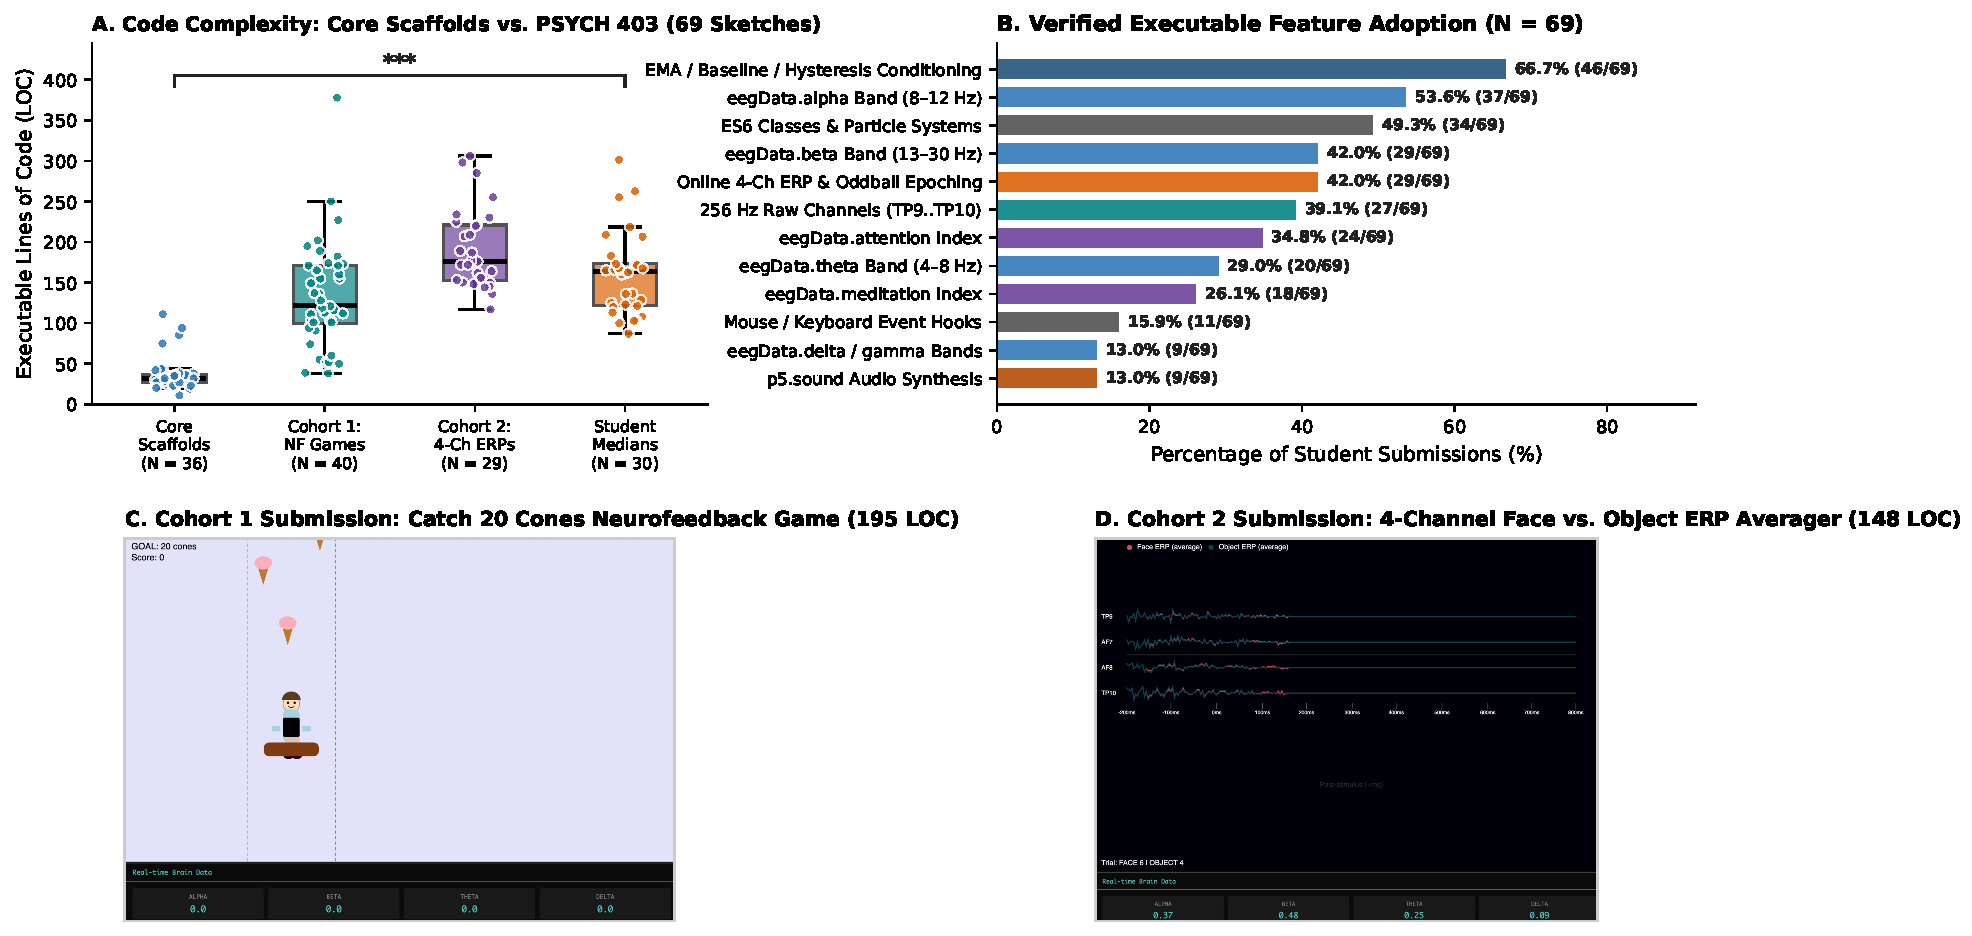
\includegraphics[width=0.98\textwidth]{figures/fig5_psych403_student_submissions_analysis.pdf}
\caption{\textbf{Classroom Evaluation of $N = \NStudentSketches$ Undergraduate Student Projects from $N_{\text{students}} = \NUniqueStudents$ Learners in \texttt{PSYCH 403}.} \textbf{(A)} Executable Lines of Code (LOC) comparing BrainImation's introductory scaffolds ($N = \NBuiltinExamples$, median $\ExLOCMedian\text{ LOC}$) against Student Cohort~1 (Neurofeedback Games \& Art; $N = \NStuNF$, median $\StuNFLOCMedian\text{ LOC}$), Student Cohort~2 (Online 4-Channel ERP Experiments; $N = \NStuERP$, median $\StuERPLOCMedian\text{ LOC}$), and per-student median lengths ($N_{\text{students}} = \NUniqueStudents$, median $\StuClusterLOCMedian\text{ LOC}$, $\text{IQR} = \StuClusterLOCIQRLow\text{--}\StuClusterLOCIQRHigh\text{ LOC}$, Mann--Whitney $U = \MannWhitneyClusterU, p < 10^{-11}, r_{rb} = \RankBiserialClusterR$). \textbf{(B)} Percentage of student submissions using signal conditioning ($\StuPctCond\%$, $\StuCntCond/\NStudentSketches$; Cohort~1: $\NFPctCond\%$, Cohort~2: $\ERPPctCond\%$), alpha ($\NFPctAlpha\%$ of Cohort~1, $\StuPctAlpha\%$ overall), beta ($\NFPctBeta\%$ of Cohort~1, $\StuPctBeta\%$ overall), attention ($\NFPctAtt\%$ of Cohort~1, $\StuPctAtt\%$ overall), custom object/particle classes ($\NFPctParticles\%$ of Cohort~1, $\ERPPctParticles\%$ of Cohort~2), online ERP state machines ($100.0\%$ of Cohort~2, $\StuPctERP\%$ overall), and 256~Hz raw electrode arrays ($\ERPPctRaw\%$ of Cohort~2, $\StuPctRaw\%$ overall). \textbf{(C)} Example Cohort~1 student neurofeedback game (\emph{Catch 20 Cones}, 195~LOC), showing the falling ice-cream cone sprite, horizontal catcher paddle, score/timer HUD, and bottom alpha/beta target zone indicator bar. \textbf{(D)} Example Cohort~2 student 4-channel Face vs.\ Object ERP experiment (148~LOC), showing the four color-coded electrode traces (\texttt{TP9}, \texttt{AF7}, \texttt{AF8}, \texttt{TP10}), real-time condition waveforms, and trial counter.}
\label{fig:students}
\end{figure}

\section{Classroom Evaluation}

\subsection{Course Context \& Workflow}

\subsubsection{Participant Pool \& Ethics}
To evaluate how undergraduate neuroscience and psychology students used BrainImation in an authentic classroom setting, we analyzed all verified unique examination projects from an upper-level cognitive neuroscience laboratory course at the University of Alberta (Table~\ref{tab:corpus} and Figure~\ref{fig:students}; $N = \NStudentSketches$ submissions from $N_{\text{students}} = \NUniqueStudents$ learners in \texttt{PSYCH 403}, Research Ethics Board Protocol \texttt{Pro00050069}). Because some students saved multiple iterative versions of their work (such as an early draft alongside a final revised submission), we report both the full submission pool and a per-student clustered summary that reduces each student's work to a single median value so that every learner contributes equally to the statistical comparison.

\subsubsection{Lab-to-Home-to-Lab Cycle}
Most students enrolled in the course had little or no prior programming experience \citep{hatton2023quantitative,smith2024lowcost,iemi2026icancode}. Instruction followed a three-step weekly cycle inspired by simulation-driven experiment building \citep{deleeuw2023simulating}: during in-person laboratory sessions, students first explored and modified the short built-in starter templates while wearing physical Muse headbands; at home on their personal laptops, they built and debugged their own assignment code using the built-in signal simulator (testing game states with the Attention and Meditation sliders and verifying trial averaging on simulated ERP peaks; \texttt{EEGSimulator}); finally, they returned to the teaching lab to test their finished programs on live headbands and submitted playable web links so the instructor and teaching assistants could open, run, and grade each project directly in the browser (\texttt{?sketch=}).

\subsubsection{Two-Cohort Exam Structure}
Each student completed two graded practical coding examinations over the semester: an interactive frequency-band neurofeedback game or visualizer in the first midterm module and an online 4-channel event-related potential experiment in the second midterm module (Cohort~1: $N = \NStuNF$; Cohort~2: $N = \NStuERP$).

\begin{table}[t!]
\centering
\caption{\textbf{Summary of Code Length and Modalities Across BrainImation's \NCatalogueSketches-Sketch Visual Catalogue and $N = \NStudentSketches$ Undergraduate Student Examination Projects ($N_{\text{students}} = \NUniqueStudents$ Students in \texttt{PSYCH 403}).} Note: The $N = \NStudentSketches$ graded examination projects (Cohort~1 $N = \NStuNF$; Cohort~2 $N = \NStuERP$) are preserved alongside \NAdditionalSketches\ additional course and laboratory sketches inside the \NNeurotechCatalogue-sketch \emph{2025 Neurotech Class Catalogue}.}
\label{tab:corpus}
\footnotesize
\setlength{\tabcolsep}{3.8pt}
\resizebox{\textwidth}{!}{%
\begin{tabular}{lcccccl}
\toprule
\textbf{Catalogue Group / Student Cohort} & \textbf{$N$} & \textbf{Med.\ LOC} & \textbf{IQR LOC} & \textbf{Min--Max} & \textbf{Primary Signals Used} & \textbf{Project Type} \\
\midrule
One-Sensor Starters \& Diagnostics & \NStarterDiag & \StarterDiagLOCMedian & $\StarterDiagLOCIQRLow\text{--}\StarterDiagLOCIQRHigh$ & $\StarterDiagLOCMin\text{--}\StarterDiagLOCMax$ & Single-sensor, 16-ch Athena & Minimal starters \& hardware checks \\
Core 10-Category Scaffolds & \NBuiltinExamples & \ExLOCMedian & $\ExLOCIQRLow\text{--}\ExLOCIQRHigh$ & $\ExLOCMin\text{--}\ExLOCMax$ & EEG bands, Att/Med, 256~Hz raw & Short introductory teaching templates \\
PPG, fNIRS, IMU \& Multimodal Studios & \NStudiosGroup & \StudiosLOCMedian & $\StudiosLOCIQRLow\text{--}\StudiosLOCIQRHigh$ & $\StudiosLOCMin\text{--}\StudiosLOCMax$ & 64~Hz PPG/fNIRS, 8/20~mm, 6-DOF IMU & Step-by-step optical \& motion lessons \\
BrainGames, EEGEdu \& Classic \texttt{p5.eegedu} & \NGamesAndEEGEdu & \GamesEEGEduLOCMedian & $\GamesEEGEduLOCIQRLow\text{--}\GamesEEGEduLOCIQRHigh$ & $\GamesEEGEduLOCMin\text{--}\GamesEEGEduLOCMax$ & Closed-loop bands, SSVEP, ERP & 14 arcade games + 29 lab modules \\
Archival Class Galleries (2022 \& 2025) & \NArchivalTotal & \ArchivalLOCMedian & $\ArchivalLOCIQRLow\text{--}\ArchivalLOCIQRHigh$ & $\ArchivalLOCMin\text{--}\ArchivalLOCMax$ & Student BCI \& NeuroArt sketches & Playable past student projects \\
\textbf{Full Visual Catalogue (\texttt{manifest.json})} & \textbf{\NCatalogueSketches} & \textbf{\CatLOCMedian} & \textbf{$\CatLOCIQRLow\text{--}\CatLOCIQRHigh$} & \textbf{$\CatLOCMin\text{--}\CatLOCMax$} & \textbf{\NCatalogueCategories\ categories with thumbnails} & \textbf{Complete in-browser sketch library} \\
\midrule
Exam Cohort 1: Neurofeedback \& Games & \NStuNF & \StuNFLOCMedian & $\StuNFLOCIQRLow\text{--}\StuNFLOCIQRHigh$ & $\StuNFLOCMin\text{--}\StuNFLOCMax$ & \texttt{eegData.alpha}, \texttt{beta}, \texttt{attention} & Student neurofeedback games \& art \\
Exam Cohort 2: Online 4-Ch ERP Tasks & \NStuERP & \StuERPLOCMedian & $\StuERPLOCIQRLow\text{--}\StuERPLOCIQRHigh$ & $\StuERPLOCMin\text{--}\StuERPLOCMax$ & 256~Hz \texttt{TP9, AF7, AF8, TP10} & Oddball P300, Face N170, Stroop, MMN \\
Per-Student Clustered Medians & \NUniqueStudents & \StuClusterLOCMedian & $\StuClusterLOCIQRLow\text{--}\StuClusterLOCIQRHigh$ & $\StuClusterLOCMin\text{--}\StuClusterLOCMax$ & One median value per student & Independent student-level summary \\
\textbf{All Exam Submissions Combined} & \textbf{\NStudentSketches} & \textbf{\StuLOCMedian} & \textbf{$\StuLOCIQRLow\text{--}\StuLOCIQRHigh$} & \textbf{$\StuLOCMin\text{--}\StuLOCMax$} & \textbf{Smoothing (\StuPctCond\%), $\alpha$ (\StuPctAlpha\%), ERP (\StuPctERP\%)} & \textbf{Graded \texttt{PSYCH 403} exam archive} \\
\bottomrule
\end{tabular}%
}
\end{table}

\subsection{Code Complexity \& Scaffold Expansion}

\subsubsection{Executable LOC Metric \& Clustering}
We quantified program size using executable lines of JavaScript code, excluding blank lines and comments (lines starting with \texttt{//}, \texttt{/*}, \texttt{*}, or \texttt{*/}). Across both examination modules, students began from the brief introductory templates and authored substantially larger, self-contained applications (Figure~\ref{fig:students}A; $\text{median} = \StuLOCMedian\text{ LOC}$, $\text{IQR} = \StuLOCIQRLow\text{--}\StuLOCIQRHigh\text{ LOC}$, range $\StuLOCMin\text{--}\StuLOCMax\text{ LOC}$ vs.\ starter scaffold $\text{median} = \ExLOCMedian\text{ LOC}$; Mann--Whitney $U = \MannWhitneyU, p < 10^{-15}$). Collapsing multiple submissions from the same student into a single per-learner median confirmed a fivefold expansion above the starter templates ($N_{\text{students}} = \NUniqueStudents$, $\text{median} = \StuClusterLOCMedian\text{ LOC}$, $\text{IQR} = \StuClusterLOCIQRLow\text{--}\StuClusterLOCIQRHigh\text{ LOC}$, range $\StuClusterLOCMin\text{--}\StuClusterLOCMax\text{ LOC}$, $U = \MannWhitneyClusterU, p < 10^{-11}, r_{rb} = \RankBiserialClusterR$).

\subsubsection{Cohort 1 \& Cohort 2 Exemplars}
In the first midterm cohort, students created original closed-loop games such as an \emph{Ice Cream Cone Catcher} steered by alpha/beta target zones and an \emph{EEG Flappy Bird} with adaptive difficulty (Figure~\ref{fig:students}C; Cohort~1 $\text{median} = \StuNFLOCMedian\text{ LOC}$, exemplars: 195 and 160~LOC). In the second midterm cohort, students expanded the ERP starter template into complete two-condition experiments comparing target versus standard oddball stimuli or Face versus Object N170 responses across all four electrodes (Figure~\ref{fig:students}D; Cohort~2 $\text{median} = \StuERPLOCMedian\text{ LOC}$, exemplar: 148~LOC; \texttt{epochs.js}).

\subsubsection{Template Expansion Test}
Notably, every single student project in the ERP cohort exceeded the 85-line starter template, typically doubling its length by adding multi-condition stimulus schedules, condition-specific running averages, custom legends, and statistical summary displays ($29/29 = 100\%$, median $\EpochsExpansionFactor\times$ code expansion, range $\StuERPLOCMin\text{--}\StuERPLOCMax\text{ LOC}$, Wilcoxon signed-rank $W = \WilcoxonEpochsW, p = \WilcoxonEpochsP$; \texttt{epochs.js}).

\subsection{Disaggregated Feature Adoption}

\subsubsection{Signal Conditioning}
Inspecting student code across the two midterm assignments shows how learners selected signal-processing tools suited to each neuroscience paradigm (Figure~\ref{fig:students}B). Two-thirds of all student projects included explicit signal conditioning (e.g., moving-average smoothing, pre-stimulus baseline subtraction, or threshold hold timers), with especially high adoption in the ERP cohort ($\StuPctCond\%$, $\StuCntCond/\NStudentSketches$ overall; Cohort~1: $\NFPctCond\%$, $\NFCntCond/\NStuNF$; Cohort~2: $\ERPPctCond\%$, $\ERPCntCond/\NStuERP$).

\subsubsection{Cohort 1 Frequency-Band Usage}
Continuous frequency-band powers, attention scores, and custom object-oriented particle classes were the primary building blocks in the first cohort's neurofeedback games (alpha: $\NFPctAlpha\%$, $\NFCntAlpha/\NStuNF$; beta: $\NFPctBeta\%$, $\NFCntBeta/\NStuNF$; attention: $\NFPctAtt\%$, $\NFCntAtt/\NStuNF$; ES6 classes/particles: $\NFPctParticles\%$, $\NFCntParticles/\NStuNF$; see Figure~\ref{fig:students}B caption).

\subsubsection{Cohort 2 Buffer Usage}
By contrast, time-domain buffer operations defined the second cohort, where every project implemented a multi-trial ERP averaging state machine and nearly all projects indexed directly into the 256~Hz raw four-channel electrode arrays, with one-fifth also defining custom object classes to manage stimulus trials (ERP state machines: $100.0\%$, $\StuCntERP/\NStuERP$; 256~Hz raw arrays: $\ERPPctRaw\%$, $\ERPCntRaw/\NStuERP$; ES6 trial classes: $\ERPPctParticles\%$, $\ERPCntParticles/\NStuERP$).

\subsubsection{Archival Preservation}
All graded examination projects are preserved alongside additional laboratory exercises inside the Visual Catalogue's classroom galleries, giving future neuroscience and psychology students a growing library of playable peer examples ($N = \NStudentSketches$ exam projects plus \NAdditionalSketches\ lab sketches in the \NNeurotechCatalogue-sketch 2025 Neurotech gallery, alongside \NNeuroArtGallery\ projects in the 2022 NeuroArt gallery).

\section{Discussion}

\subsection{Pedagogical \& Research Synthesis}

\subsubsection{From Dashboards to Creative Coding}
BrainImation offers neuroscience and psychology lecturers a practical, zero-install browser environment for both undergraduate laboratory instruction and rapid behavioral research prototyping. Whereas companion dashboard tools such as \emph{EEGEdu} (\url{https://eegedu.com}) \citep{mathewson2026eegedu} introduce brain waves and frequency spectra through pre-built charts, BrainImation empowers students and researchers to write their own interactive programs driven by live EEG rhythms, time-locked ERP epochs, forehead optical blood-flow signals (PPG/fNIRS), and 3D head motion \citep{papert1980mindstorms,resnick2009scratch,deleeuw2015jspsych,henninger2022labjs}. In doing so, it bridges browser-based behavioral experiment builders \citep{woods2015conducting,dalmaijer2022mouseview,pronk2023jsquestplus,deleeuw2024datapipe} and hands-on undergraduate neurophysiology curricula \citep{janssen2021opportunities,hatton2023quantitative,smith2024lowcost,iemi2026icancode}.

\subsubsection{Zero-Install Lab \& Off-Lab Workflow}
By supporting all four Muse headset generations through a single browser button, providing a realistic multi-sensor simulator for homework and lecture demonstrations \citep{deleeuw2023simulating}, and pairing a \NRefAPIs-item Reference Drawer with a \NCatalogueSketches-sketch Visual Catalogue, the platform shifts classroom time away from software installation and driver troubleshooting toward experimental design, physiological signal interpretation, and joint neurocognitive modeling \citep{frischkorn2018cognitive,schubert2023enhancing,nunez2024tutorial,dekleijn2025phasic}. When students are ready to transition from in-browser prototyping to advanced offline pipelines, one-click CSV export connects seamlessly with open-source Python, R, and MATLAB ecosystems including EEGLAB \citep{delorme2004eeglab}, \texttt{BrainBeats} \citep{cannard2024brainbeats}, \texttt{NeuroKit2} \citep{makowski2021neurokit2}, the Lab Streaming Layer \citep{kothe2025lsl}, and synchronous multimodal web viewers \citep{pijalek2026meedav}.

\subsection{Technical \& Methodological Limitations}

\subsubsection{Synthetic Benchmarks vs.\ Clinical Validation}
When adopting BrainImation in a course or laboratory, several practical boundaries are helpful to keep in mind. First, the simulation benchmarks in Section~4 (Figures~\ref{fig:sonification} and \ref{fig:multimodal}) test in-browser algorithms on repeatable synthetic signals with known ground truth; they are designed as clear teaching demonstrations rather than clinical hardware validations against research-grade fNIRS systems or wet-electrode EEG caps \citep{cannard2021validating,sabio2024scoping,vanbueren2026comparing,russo2025fnirs}. In classroom ERP and spectral labs, instructors can also have students compute the trial-to-trial Standardized Measurement Error (SME; \citealp{luck2021standardized,schubert2023enhancing}), inspect the $1/f^{\chi}$ aperiodic slope alongside narrowband alpha power \citep{vanbueren2026comparing}, and test heartbeat-locked averages against surrogate pseudotrial permutations \citep{steinfath2025validating} so students learn rigorous modern reporting standards \citep{picton2000guidelines,keil2014committee}.

\subsubsection{WebBluetooth \& 60~Hz Jitter}
Second, because Bluetooth packets arrive in small bursts and browser animation loops redraw the screen at 60 frames per second ($16.67\text{ ms}$ per frame), visual stimulus timestamps in browser ERP tasks have $\sim 15\text{--}45\text{ ms}$ of frame-to-frame timing variability compared with dedicated laboratory trigger cables \citep{krigolson2017choosing,kuziek2017transitioning,kuziek2018increasing,pronk2020mental,anwyl2021realistic,lukacs2023precise}. As quantified in Figure~\ref{fig:sonification}E, averaging across trials with slight timing jitter acts like a gentle temporal smoothing filter: it attenuates very brief sensory spikes ($<20\text{ ms}$ wide) but preserves broader cognitive waves such as the N170 face response and the P300 oddball response across 20 averaged trials ($30\text{ ms}$ [$45\text{ ms}$] uniform jitter low-pass cutoff: $f_c = \JitterFCThirtyHz\text{ Hz}$ [$\JitterFCFortyFiveHz\text{ Hz}$], first spectral null at $\JitterNullThirtyHz\text{ Hz}$ [$\JitterNullFortyFiveHz\text{ Hz}$]; amplitude retained under $30\text{ ms}$ jitter: $\JitterRetNarrowPct\%$ for a narrow $20\text{ ms}$ peak vs.\ $\JitterRetNOneSeventyPct\%$ for N170 and $\JitterRetPThreeHundredPct\%$ for P300), especially when paired with fractional-area or dynamic template-matching latency estimators \citep{schubert2024multiverse,schubert2026dynamic}.

\subsubsection{Dry-Sensor Artifacts \& NLMS Bounds}
Third, dry forehead and behind-the-ear sensors are naturally sensitive to eye blinks, forehead or jaw muscle tension, and mechanical headband slippage \citep{lotte2013flaws,mathewson2017high,saager2005direct,wyser2020short}. Although the built-in amplitude-rejection threshold, short-channel optical regression, and 6-axis adaptive motion filter provide effective classroom demonstrations of artifact removal, our viscoelastic lag benchmark (Figure~\ref{fig:multimodal}F) illustrates why the default 1-tap-per-axis filter is best suited for synchronous movement swings, whereas multi-tap delayed FIR reference vectors are advantageous during ambulatory tasks with slow mechanical electrode settling \citep{rosanne2021adaptive,klug2022bemobil}.

\subsubsection{Browser Compatibility}
Fourth, connecting a physical Muse headband via WebBluetooth requires a Chromium-based browser (such as Google Chrome, Microsoft Edge, Opera, or the Bluefy browser on iOS and iPadOS). However, the built-in signal simulator, code editor, Reference Drawer, and Visual Catalogue work in any modern browser, including Safari and Firefox, so students on any laptop or tablet can complete homework and explore every example.

\subsubsection{Classroom Evaluation Scope}
Finally, our classroom evaluation measured program complexity and feature adoption across $N = \NStudentSketches$ graded student projects rather than pre- and post-course quiz scores. Because students could build upon catalogue templates and use AI coding explanations \citep{clindeffarges2026socrates}, program length reflects the scope of the interactive experiments students constructed rather than memorized syntax. Together, these features make BrainImation an approachable, zero-install bridge between introductory neuroscience demonstrations and hands-on computational experimentation.

\subsection*{Declarations}
\noindent\textbf{Open Practices Statement:} All source code (\texttt{muse-browser.js}, \texttt{index.html}, Python \texttt{bleak} hardware diagnostics in \texttt{tools/}), the live browser environment (\url{https://kylemath.github.io/Brainimation/}), all \NCatalogueSketches\ catalogue sketches and thumbnails in \texttt{examples/}, simulation benchmark generators, and the automated manuscript verification suite (\texttt{verify\_manuscript\_analyses.py}) are openly available without restriction at \url{https://github.com/kylemath/Brainimation} and \url{https://github.com/kylemath/eegeduPaper}. The classroom evaluation analyzed de-identified archival student code rather than a preregistered hypothesis test.\\[2pt]
\noindent\textbf{Ethics and SAGER Statement:} Classroom code artifacts from \texttt{PSYCH 403} were analyzed in de-identified form in accordance with procedures approved by the University of Alberta Research Ethics Board (Protocol \texttt{Pro00050069}). Because software source files were analyzed in de-identified archival form without demographic linkage, participant sex and gender dimensions were not recorded and do not affect the deterministic signal-processing benchmarks.\\[2pt]
\noindent\textbf{Data and Code Availability:} The live BrainImation environment is available at \url{https://kylemath.github.io/Brainimation/}. Source code and analysis scripts are archived at \url{https://github.com/kylemath/Brainimation} and \url{https://github.com/kylemath/eegeduPaper}.\\[2pt]
\noindent\textbf{Funding:} This work was supported by a Natural Sciences and Engineering Research Council of Canada (NSERC) Discovery Grant to K.E.M. The funding source had no involvement in study design; in the collection, analysis, and interpretation of data; in the writing of the report; or in the decision to submit the article for publication.\\[2pt]
\noindent\textbf{Declaration of Competing Interest:} The authors declare that there are no known competing financial interests or personal relationships that could have appeared to influence the work reported in this paper.\\[2pt]
\noindent\textbf{CRediT Authorship Contribution Statement:} \textbf{Kyle E. Mathewson:} Conceptualization, Methodology, Software, Validation, Formal analysis, Investigation, Resources, Data curation, Writing -- original draft, Writing -- review \& editing, Visualization, Supervision, Project administration, Funding acquisition. \textbf{Tamari Shalamberidze:} Methodology, Software, Validation, Investigation, Data curation, Writing -- review \& editing. \textbf{Claire J. Scavuzzo:} Conceptualization, Methodology, Investigation, Supervision, Writing -- review \& editing.\\[2pt]
\noindent\textbf{Declaration of Generative AI and AI-Assisted Technologies in the Manuscript Preparation Process:} During the preparation of this work the authors used large language model coding and editing assistants to verify code-to-manuscript consistency and polish prose formatting. After using these tools, the authors reviewed and edited the content as needed and take full responsibility for the content of the published article.\\[2pt]
\noindent\textbf{Acknowledgements:} The authors thank the undergraduate students and teaching assistants of \texttt{PSYCH 403} and the NeuroArt and Neurotech laboratory cohorts at the University of Alberta for testing BrainImation in the classroom.

\bibliographystyle{apalike}
\bibliography{references2}

\end{document}
